\documentclass[9pt]{beamer}
\usepackage[utf8]{inputenc}
\usepackage[russian,english]{babel}
\usepackage{graphicx, epsfig}
\usepackage{amsmath,mathrsfs,amsfonts,amssymb}
\usepackage{subfig}
\usepackage{floatflt}
\usepackage{epic,ecltree}
\usepackage{mathtext}
\usepackage{fancybox}
\usepackage{fancyhdr}
\usepackage{multirow}
\usepackage{enumerate}
\usepackage{epstopdf}
\usepackage{multicol}
\usepackage{algorithm}
\usepackage[noend]{algorithmic}
\def\algorithmicrequire{\textbf{Input:}}
\def\algorithmicensure{\textbf{Output:}}
\usetheme{Singapore}%{Singapore}%{Warsaw}%{Warsaw}%{Darmstadt}
\usecolortheme{default}
\setbeamertemplate{footline}[page number]{}
\newcommand{\bx}{\mathbf{x}}
\newcommand{\by}{\mathbf{y}}
\newcommand{\bz}{\mathbf{z}}
\newcommand{\bw}{\mathbf{w}}
\newcommand{\ba}{\mathbf{a}}
\newcommand{\bb}{\mathbf{b}}
\newcommand{\bY}{\mathbf{Y}}
\newcommand{\bX}{\mathbf{X}}
\newcommand{\bu}{\mathbf{u}}
\newcommand{\bt}{\mathbf{t}}
\newcommand{\bp}{\mathbf{p}}
\newcommand{\bq}{\mathbf{q}}
\newcommand{\bc}{\mathbf{c}}
\newcommand{\bP}{\mathbf{P}}
\newcommand{\bT}{\mathbf{T}}
\newcommand{\bB}{\mathbf{B}}
\newcommand{\bQ}{\mathbf{Q}}
\newcommand{\bC}{\mathbf{C}}
\newcommand{\bE}{\mathbf{E}}
\newcommand{\bF}{\mathbf{F}}
\newcommand{\bU}{\mathbf{U}}
\newcommand{\bW}{\mathbf{W}}
\newcommand{\bbR}{\mathbb{R}}
\newcommand{\cA}{\mathcal{A}}
\newcommand{\bchi}{\boldsymbol{\chi}}
\newcommand{\bphi}{\boldsymbol{\phi}}
\newcommand{\btheta}{\boldsymbol{\theta}}
\newcommand{\bTheta}{\boldsymbol{\Theta}}
\newcommand{\argmin}{\mathop{\arg \min}\limits}
\newcommand{\argmax}{\mathop{\arg \max}\limits}

\newcommand\undermat[2]{%
	\makebox[0pt][l]{$\smash{\underbrace{\phantom{%
					\begin{matrix}#2\end{matrix}}}_{\text{$#1$}}}$}#2}

\newtheorem{statement}{Statement}

\usepackage{tikz-cd}
%\definecolor{beamer@blendedblue}{RGB}{15,120,80}
%----------------------------------------------------------------------------------------------------------
\title[\hbox to 56mm{  \hfill\insertframenumber\,/\,\inserttotalframenumber}]
{\\ \vspace{1.5cm} Dimensionality reduction for signal forecasting}
\author[Roman Isachenko]{\\ 
	\vspace{.4cm}
	Roman Isachenko}
\institute[SkolTech]{Skoltech advisor: Maxim Fedorov \\ 
	\vspace{0.1cm}
	 MIPT advisor: Vadim Strijov
}
\date{April 18, 2018.}
%--------------------------------------------------------------------------------
\begin{document}
%--------------------------------------------------------------------------------
\begin{frame}
%\thispagestyle{empty}
\titlepage
\end{frame}
%--------------------------------------------------------------------------------
\begin{frame}{General Problem}
	\begin{block}{Task}
		To analyze the input signal.
		\begin{itemize}
			\item multicollinearity in input and target spaces;
			\item high correlation between signals;
			\item the covariance matrices are essentially non-diagonal.
		\end{itemize}
	There are two models for input and target spaces. 
	\end{block}
	\begin{block}{Goal}
		To adjust the models for high multicollinear spaces.
	\end{block}
	\begin{block}{Problem}
		To select structurally simple, stable, and exact model in the case of data redundancy and multiextremality of an error function.
	\end{block}
	\begin{block}{Solution}
		Feature selection method that takes into account the input and target spaces structures and gives self-consistent model.
	\end{block}
\end{frame}
%--------------------------------------------------------------------------------
\begin{frame}{Literature}
	\begin{itemize}
		\item Katrutsa A., Strijov V. Comprehensive study of feature selection methods to solve multicollinearity problem according to evaluation criteria. // \textit{Expert Systems with Applications} 76, 2017.
		\vfill
		\item Eliseyev A., Aksenova T. Stable and artifact-resistant decoding of 3D hand trajectories from ECoG signals using the generalized additive model //\textit{Journal of neural engineering} 11(6), 2014.
		\vfill
		\item Eliseyev A. et al. Iterative N-way partial least squares for a binary self-paced brain–computer interface in freely moving animals //\textit{Journal of neural engineering} 4(8), 2011.
		\vfill
		\item Rodriguez-Lujan I. et al. Quadratic programming feature selection // \textit{Journal of Machine Learning Research} 11(Apr), 2010.
		\vfill
		\item Motrenko A., Strijov V. Multi-way Feature Selection for ECoG-based Brain-Computer Interface // \textit{Expert Systems with Applications} Submitted to the journal.
	\end{itemize}
\end{frame}
%--------------------------------------------------------------------------------
\begin{frame}{Application: Brain Computer Interface (BCI)}
\begin{minipage}{0.45\linewidth}
	\begin{figure}
		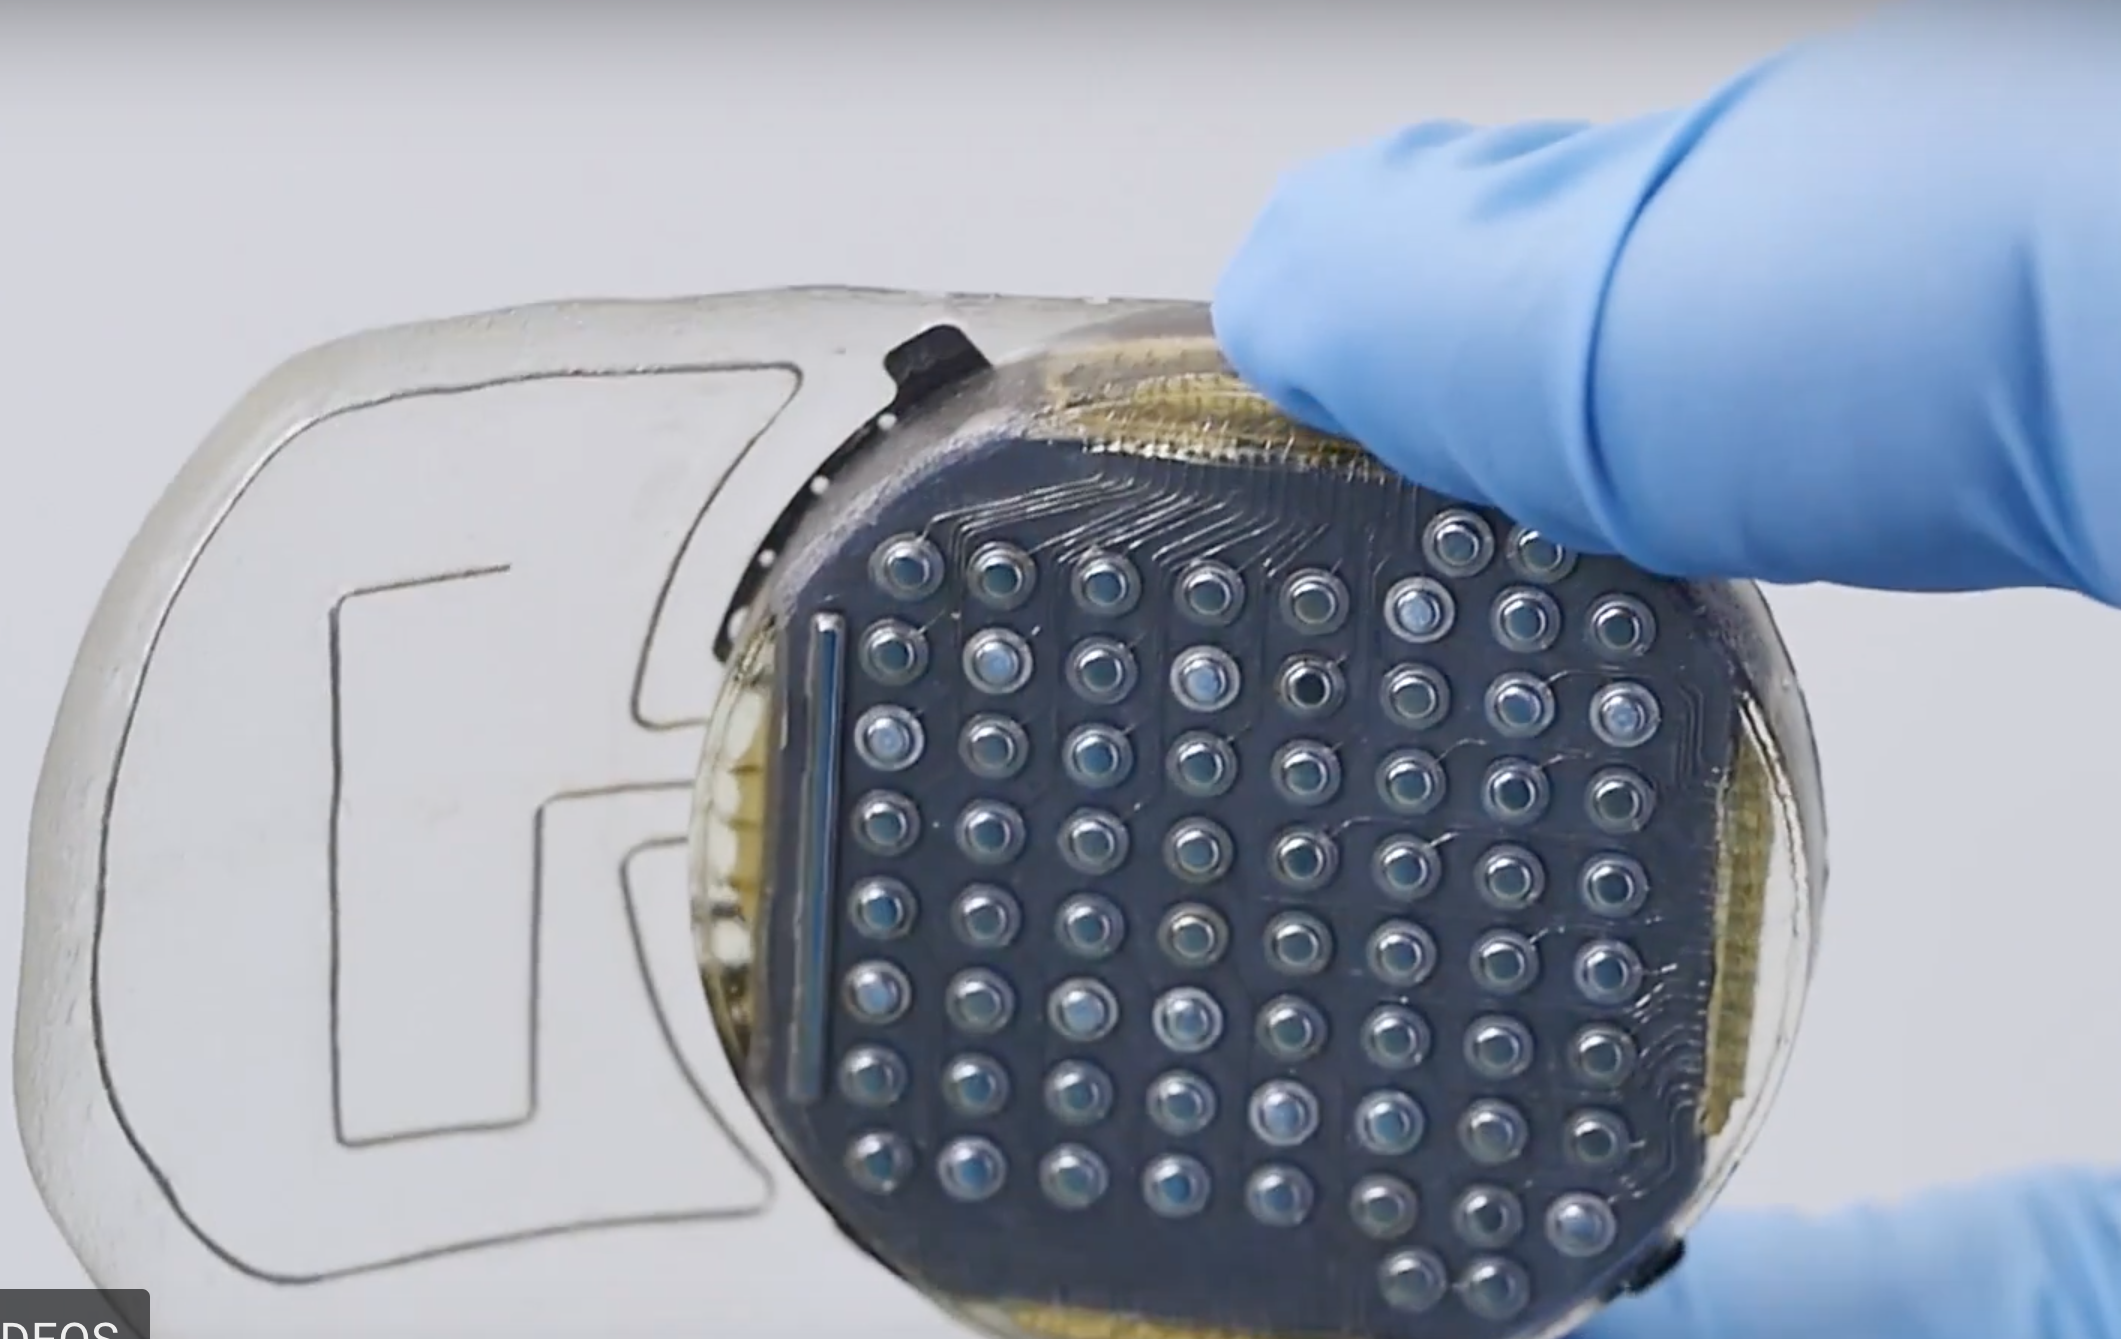
\includegraphics[width=0.96\linewidth]{figs/deviceClinatec} \\
		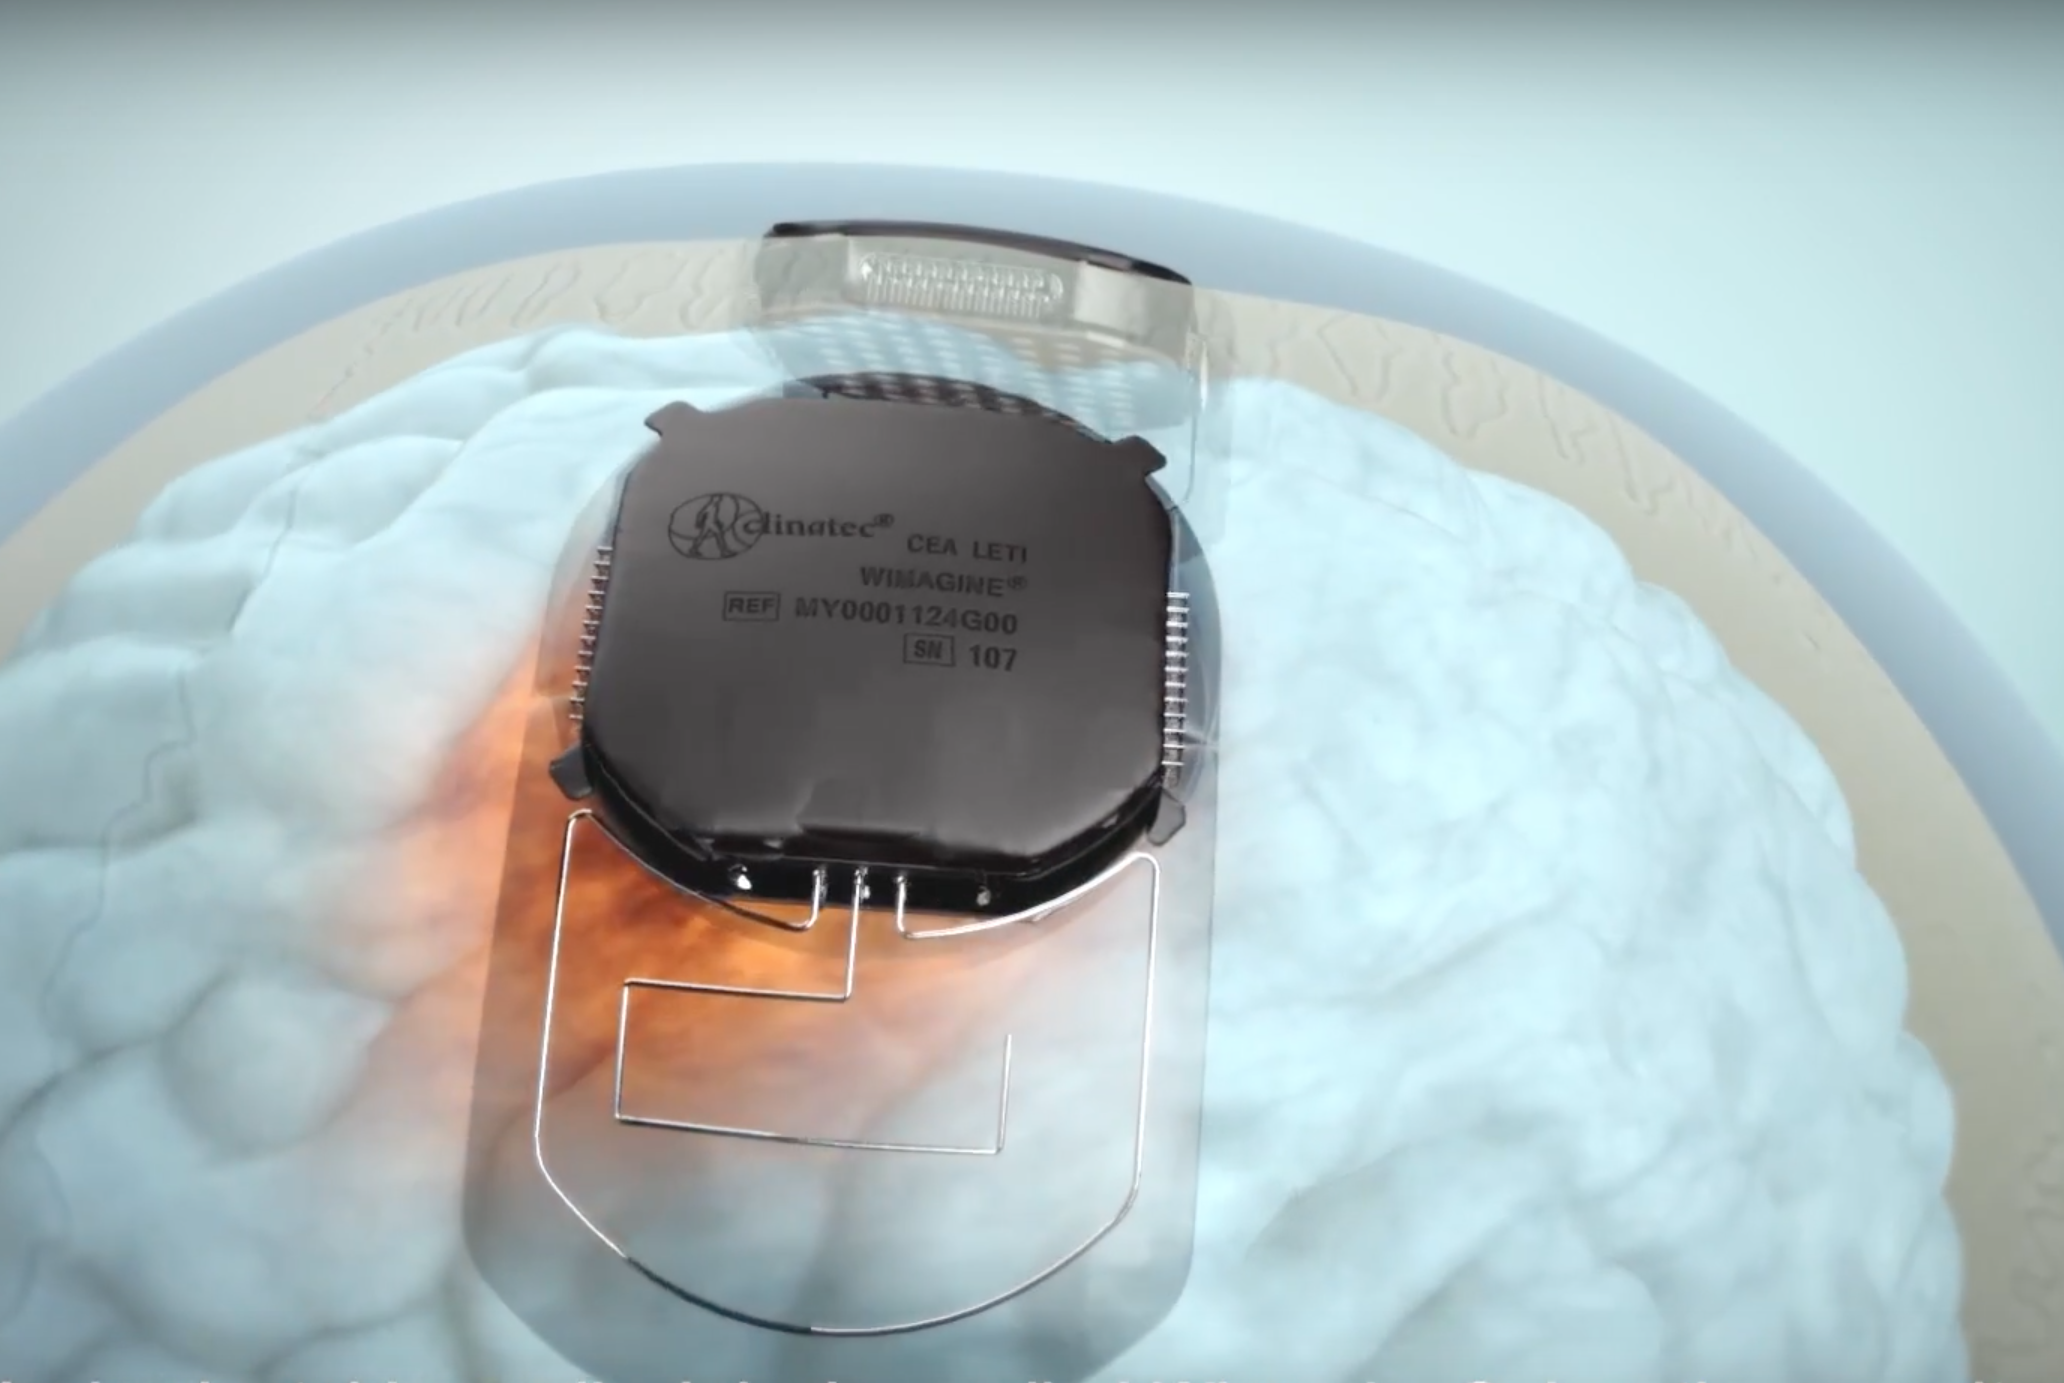
\includegraphics[width=0.96\linewidth]{figs/brainClinatec}
	\end{figure}
\end{minipage}%
\begin{minipage}{0.55\linewidth}
	\centering
	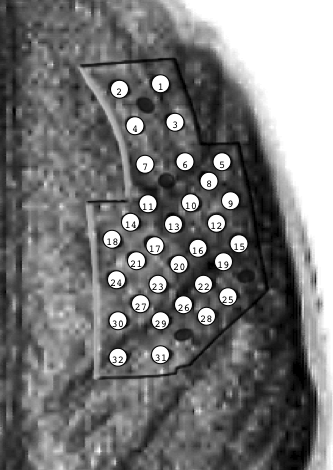
\includegraphics[width=0.73\linewidth]{figs/electrodes}
\end{minipage}
\vspace{0.1cm} \\
\hrulefill \\
\url{http://clinatec.fr}; 
\url{http://neurotycho.org}
\end{frame}
%--------------------------------------------------------------------------------
\begin{frame}{Problem Statement}
	\begin{block}{Goal}
	Forecast a dependent variable $\by \in \bbR^r$ from an independent input object $\bx \in \bbR^n$.
	\[
	\by = \bTheta \bx+ \boldsymbol{\varepsilon}, \quad \bTheta \in \bbR^{r \times n}
	\]
	\vspace{-0.7cm}
	\end{block}
	\begin{block}{Given}
	Dataset $\left( \bX, \bY \right)$, where $\bX \in \bbR^{m \times n}$ is a design matrix, $\bY \in \bbR^{m \times r}$ is a target matrix
	\[
	\bX = [\bx_1, \dots, \bx_m]^{T} =  [\bchi_1, \dots, \bchi_n]; \quad \bY = [\by_1, \dots, \by_m]^{T} =  [\bphi_1, \dots, \bphi_r].
	\]
	\vspace{-0.7cm}
	\end{block}
	\begin{block}{Error function}
	\[
	S(\bTheta | \bX, \bY) = {\left\| \underset{m \times r}{\mathbf{Y}}  - \underset{m \times n}{\bX} \cdot \underset{r \times n}{\bTheta}^T \right\| }_2^2 \rightarrow\min_{\bTheta}.
	\label{eq:error_function}
	\]
	\[
	\bTheta = (\bX^{T} \bX)^{-1} \bX^{T} \bY.
	\]
	\end{block}
	The linear dependent columns of the matrix $\bX$ leads to an instable solution. \\
	To avoid the strong linear dependence, feature selection and dimensionality reduction techniques are used.
\end{frame}

%--------------------------------------------------------------------------------
\begin{frame}{Feature Selection}
\begin{block}{Goal}
Find the index set~$\cA = \{1, \dots, n\}$ of~$\bX$ columns. 
\end{block}
\begin{block}{Quality Criteria}
To select the set~$\cA$ among all possible $2^n - 1$ subsets, introduce the feature selection quality criteria
\[
\cA = \argmax_{\cA' \subseteq \{1, \dots, n\}} Q(\cA' | \bX, \bY).
\label{eq:subset_selection}
\]
\end{block}
Once the solution~$\cA$ is known:
\[
S(\bTheta_{\cA} | \bX_{\cA}, \bY) = {\left\| \mathbf{Y} - \bX_{\cA}\bTheta^T_{\cA} \right\| }_2^2 \rightarrow\min_{\bTheta_{\cA}},
\]
where the subscript~$\cA$ indicates columns with indices from the set~$\cA$.

\end{frame}
%--------------------------------------------------------------------------------
\begin{frame}{Quadratic Programming Feature Selection}
	\[
	\| \bphi - \bX \btheta\|_2^2 \rightarrow\min_{\btheta \in \bbR^{n}}.
	\]
	\begin{block}{Quadratic Programming Feature Selection}
	\vspace{-0.3cm}
	\[
	(1 - \alpha) \cdot \underbrace{\ba^{T} \bQ \ba}_{\text{Sim}(\bX)} - \alpha \cdot \underbrace{\vphantom{()} \mathbf{b}^{T} \ba}_{\text{Rel}(\bX, \bphi)} \rightarrow \min_{\substack{\ba \in \bbR^n_+ \\ \|\ba\|_1=1}}.
	\]
	\vspace{-0.3cm}
	\end{block}
		\begin{itemize}
			\item $\ba \in \bbR^n$ --- feature importances;
			\item $\bQ \in \bbR^{n \times n}$ - pairwise feature similarities;
			\item $\mathbf{b} \in \bbR^n$ - feature relevances to the target vector.
		\end{itemize}
	
	\begin{equation*}
	j \in \mathcal{A}^* \Leftrightarrow a_j > \tau
	\end{equation*}
	
	\begin{block}{Quality Criteria}
	\[
	\cA = \argmax_{\cA' \subseteq \{1, \dots, n\}} Q(\cA' | \bX, \bphi) \Leftrightarrow \argmin_{\ba  \in \bbR^n_+, \, \|\ba\|_1=1} \bigl[\ba^{T} \bQ \ba - \alpha \cdot \mathbf{b}^{T} \ba \bigr].
	\]
	\end{block}
\end{frame}
%--------------------------------------------------------------------------------
\begin{frame}{Quadratic Programming Feature Selection}
	
	\begin{block}{Quality Criteria}
		\[
		\cA = \argmax_{\cA' \subseteq \{1, \dots, n\}} Q(\cA' | \bX, \bphi) \Leftrightarrow \argmin_{\ba  \in \bbR^n_+, \, \|\ba\|_1=1} \bigl[\ba^{T} \bQ \ba - \alpha \cdot \mathbf{b}^{T} \ba \bigr].
		\]
		\vspace{-0.5cm}
	\end{block}
	\begin{block}{Similarity measure}
		\begin{itemize}
			\item Correlation
			\vspace{-0.1cm}
			\[
			\left|\text{corr}(\bx, \by)\right| = \left| \frac{\mathrm{cov}(\bx, \by)}{\sqrt{\mathrm{Var}(\bx) \mathrm{Var}(\by)}} \right|
			\]
			\vspace{-0.3cm}
			\item Mutual information
			\vspace{-0.1cm}
			\[
			I(\bx, \by) = \int \int p(\bx, \by) \log \frac{p(\bx, \by)}{p(\bx) p(\by)} d\bx d\by.
			\]
			\vspace{-0.5cm}
		\end{itemize}
	\end{block}
	\[
	\bQ = \left\{\left|\text{corr}(\bchi_i, \bchi_j)\right|\right\}_{i,j=1}^n, \quad \bb = \left\{\left|\text{corr}(\bchi_i, \bphi)\right|\right\}_{i=1}^n.
	\]
	\vspace{-0.5cm}
	\begin{block}{Statement}
		In the case of semidefinite matrix $\bQ$ the QPFS problem is convex.
	\end{block}
	\begin{equation*}
	\bQ \rightarrow \bQ - \lambda_{\min} \mathbf{I}	
	\end{equation*}
\end{frame}
%--------------------------------------------------------------------------------
\begin{frame}{Multivariate QPFS}
\begin{block}{Relevance aggregation}
\vspace{-0.3cm}
\[
\bQ = \left\{\left|\text{corr}(\bchi_i, \bchi_j)\right|\right\}_{i,j=1}^n, \quad \bb = \left\{\sum_{k=1}^r\left|\text{corr}(\bchi_i, \bphi_k)\right|\right\}_{i=1}^n.
\]
\vspace{-0.3cm}
\end{block}

This approach does not use the dependencies in the columns of the matrix $\bY$. 
\begin{block}{Example:}
\vspace{-0.5cm}
\[
\bX = [\bchi_1, \bchi_2, \bchi_3], \quad \bY = [\underbrace{\bphi_1, \bphi_1, \dots, \bphi_1}_{r-1}, \bphi_2],
\]
\vspace{-0.2cm}
\[
\bQ = \begin{bmatrix} 1 & 0 & 0\\ 0 & 1 & 0.8 \\ 0 & 0.8 & 1 \end{bmatrix}, \quad 
\bB = \begin{bmatrix} 0.4 & \dots & 0.4 & 0 \\ 0.5 & \dots & 0.5 & 0.8 \\ \undermat{r-1}{0.8 & \dots & 0.8} & 0.1 \end{bmatrix}, \quad
\bb = \begin{bmatrix} (r-1) \cdot 0.4 + 0 \\ (r-1) \cdot 0.5 + 0.8 \\ (r-1) \cdot 0.8 + 0.1 \end{bmatrix}
\]
\end{block}
\vspace{0.2cm}

Best subset: $[\bchi_1, \bchi_2]$. \\
\vspace{0.2cm}
QPFS ($r=2$): $\ba = [\mathbf{0.37},	\mathbf{0.61},	0.02]$. \\
QPFS ($r=5$): ~$\ba = [\mathbf{0.40},	0.17, \mathbf{0.43}]$. 
\end{frame}
%--------------------------------------------------------------------------------
\begin{frame}{Multivariate QPFS}
\begin{block}{Proposal}
Penalize correlated targets by $\text{Sim} (\bY)$
\[
\alpha_1 \cdot \underbrace{\ba_x^{T} \bQ_x \ba_x}_{\text{Sim}(\bX)} - \alpha_2 \cdot \underbrace{\ba_x^{T} \bB \ba_y}_{\text{Rel}(\bX, \bY)} + \alpha_3 \cdot \underbrace{\ba_y^{T} \bQ_y \ba_y}_{\text{Sim}(\bY)} \rightarrow \min_{\substack{\ba_x \in \bbR^n_+ \, \|\ba_x\|_1=1 \\ \ba_y \in \bbR^r _+ \, \|\ba_y\|_1=1}}.
\]
\vspace{-0.5cm}
\end{block}
\[
\bQ_x = \left\{ \left| \text{corr}(\bchi_i, \bchi_j) \right| \right\}_{i,j=1}^n, \,
\bQ_y = \left\{ \left| \text{corr}(\bphi_i, \bphi_j) \right| \right\}_{i,j=1}^r, \,
\bB =  \left\{ \left| \text{corr}(\bchi_i, \bphi_j) \right| \right\}_{\substack{i=1, \dots, n \\ j=1, \dots, r}}.
\]
\[
\alpha_1 + \alpha_2 + \alpha_3 = 1 \quad \alpha_i \geq 0, \, i = 1, 2, 3.
\] 
\begin{statement}
	For the case $r=1$ the proposed functional coincides with the original QPFS algorithm.
\end{statement}

\begin{statement}
	Balance between the terms $\text{Sim}(\bX)$ and $\text{Rel}(\bX, \bY)$ for the problem is achieved by the following coefficients:
	\vspace{-0.2cm}
	\[
	\alpha_1 = \frac{(1 - \alpha_3)\overline{\bB}}{\overline{\bQ}_x + \overline{\bB}}; \quad
	\alpha_2 = \frac{(1 - \alpha_3)\overline{\bQ}_x}{\overline{\bQ}_x + \overline{\bB}}; \quad
	\alpha_3 \in [0, 1],
	\]
	where $\overline{\bQ}_x$, $\overline{\bB}$ are the mean values of~$\bQ_x$ and $\bB$ respectively.
\end{statement}
\end{frame}
%--------------------------------------------------------------------------------
\begin{frame}{Multivariate QPFS}
	\begin{block}{Example:}
		\vspace{-0.5cm}
		\[
		\bX = [\bchi_1, \bchi_2, \bchi_3], \quad \bY = [\underbrace{\bphi_1, \bphi_1, \dots, \bphi_1}_{r-1}, \bphi_2],
		\]
		\vspace{-0.2cm}
		\[
		\bQ = \begin{bmatrix} 1 & 0 & 0\\ 0 & 1 & 0.8 \\ 0 & 0.8 & 1 \end{bmatrix}, \quad 
		\bB = \begin{bmatrix} 0.4 & \dots & 0.4 & 0 \\ 0.5 & \dots & 0.5 & 0.8 \\ \undermat{r-1}{0.8 & \dots & 0.8} & 0.1 \end{bmatrix}, \quad
		\bb = \begin{bmatrix} (r-1) \cdot 0.4 + 0 \\ (r-1) \cdot 0.5 + 0.8 \\ (r-1) \cdot 0.8 + 0.1 \end{bmatrix}
		\]
	\end{block}
	\vspace{0.2cm}
	\begin{center}
$\bQ_x = \bQ$; $\bQ_y:$ $\text{corr}(\bphi_1, \bphi_2) = 0.2$ all others entries = 1. 
\end{center}
\begin{figure}
	\centering
	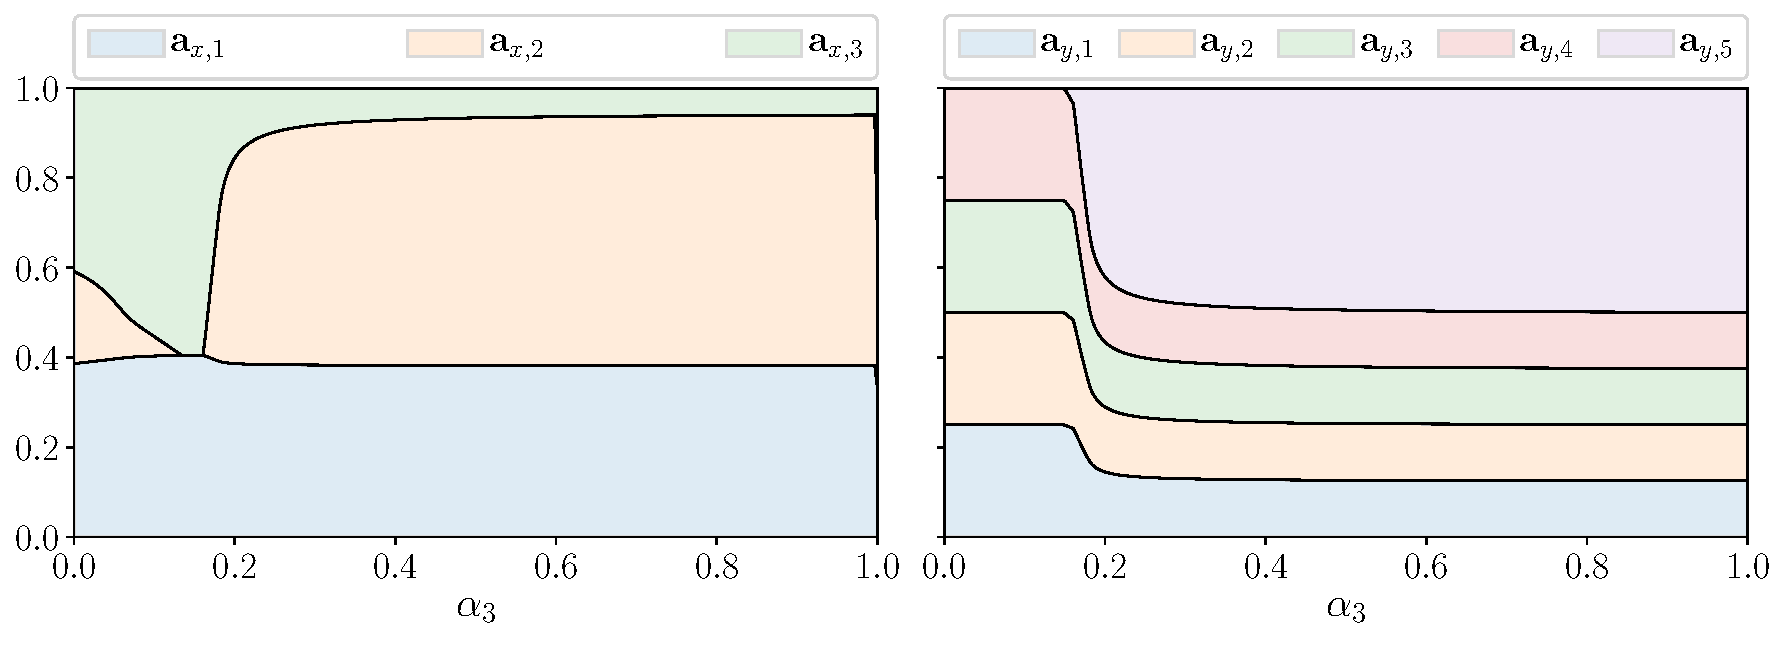
\includegraphics[width=\linewidth]{figs/features_vs_alpha.pdf}
\end{figure}
\end{frame}
%--------------------------------------------------------------------------------
\begin{frame}{Feature categorization}
\begin{enumerate}
	\item non-relevant features
	\[
	\left\{j: \text{corr}(\bchi_j, \bphi_k) = 0, \, \forall k \in \{1, \dots, r\}\right\};
	\]
	\item non-$\bX$-correlated features, which are relevant to non-$\bY$-correlated targets
	\[
	\left\{j: \left(\text{VIF}(\bchi_j) < 10\right) \, \text{and} \, \left(\text{VIF}(\bphi_k) < 10 , \, \forall k \in \{1, \dots, r\}: \,  \text{corr}(\bchi_j, \bphi_k) \neq 0 \right)\right\};
	\]
	\item non-$\bX$-correlated features, which are relevant to $\bY$-correlated targets
	\[
	\left\{j: \left(\text{VIF}(\bchi_j) < 10\right) \, \text{and} \, \left( \exists k \in \{1, \dots, r\}: \text{VIF}(\bphi_k) > 10 \,\, \& \,\, \text{corr}(\bchi_j, \bphi_k) \neq 0 \right)\right\};
	\]
	\item $\bX$-correlated features, which are relevant to non-$\bY$-correlated targets
	\[
	\left\{j: \left(\text{VIF}(\bchi_j) > 10\right) \, \text{and} \, \left(\text{VIF}(\bphi_k) < 10 , \, \forall k \in \{1, \dots, r\}: \,  \text{corr}(\bchi_j, \bphi_k) \neq 0 \right)\right\};
	\]
	\item $\bX$-correlated features, which are relevant to $\bY$-correlated targets
	\[
	\left\{j: \left(\text{VIF}(\bchi_j) > 10\right) \, \text{and} \, \left( \exists k \in \{1, \dots, r\}: \text{VIF}(\bphi_k) > 10 \,\, \& \,\, \text{corr}(\bchi_j, \bphi_k) \neq 0 \right)\right\}.
	\]
\end{enumerate}

\[
r = \text{corr} (\bchi, \bphi), \quad t = \frac{r \sqrt{m - 2}}{1 - r^2} \sim \text{St} (m - 2).
\]
\[
\text{VIF}(\bchi_j) = \frac{1}{1 - R_j^2}, \quad \text{VIF}(\bphi_k) = \frac{1}{1 - R_k^2},
\]
where $R_j^2$($R_k^2$) are coefficients of determination for the regression of $\bchi_j$($\bphi_k$) on the other features(targets).
\end{frame}
%--------------------------------------------------------------------------------
\begin{frame}{Computational experiment}
\begin{minipage}{0.55\textwidth}
	\begin{block}{Datasets}
		\vspace{0.35cm}
		\begin{itemize}
			\item energy consumption
			\item electrocorticogram signals (ECoG)
		\end{itemize}
	\end{block}
	\vspace{0.5cm}
\end{minipage}%
\begin{minipage}{0.45\textwidth}
	\begin{block}{Autoregressive approach}
		\[
		\mathbf{X} = 
		\begin{pmatrix}
		x_1 & x_2 & \dots & x_n \\
		x_2 & x_3 & \dots & x_{n+1} \\
		\dots & \dots & \dots & \dots \\
		x_{T-n+1} & x_{T-n+2} & \dots & x_T
		\end{pmatrix}
		\]
	\end{block}
\end{minipage}
\begin{block}{ECoG data}
	\begin{figure}
		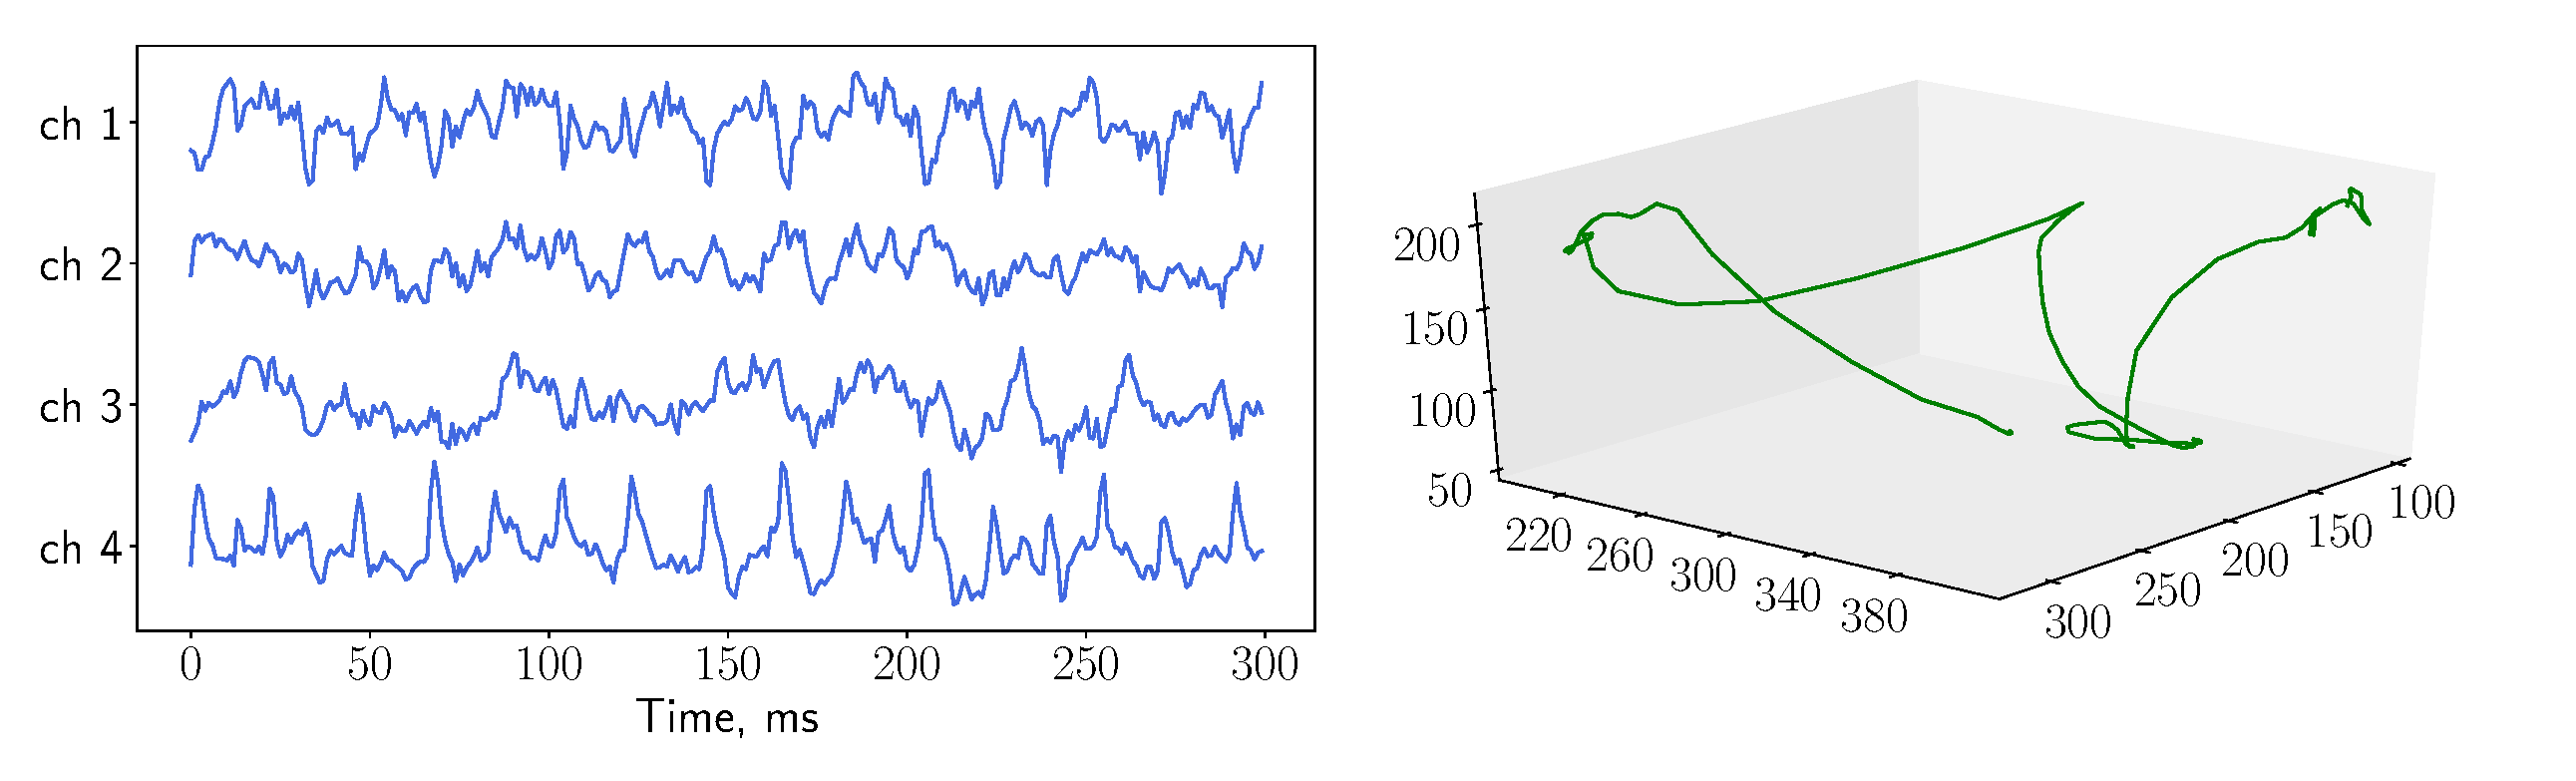
\includegraphics[width=\linewidth]{figs/ecog_data}
	\end{figure}
\end{block}
\end{frame}
%--------------------------------------------------------------------------------
\begin{frame}{Experiment}
	\begin{figure}
		\begin{minipage}{.5\linewidth}
			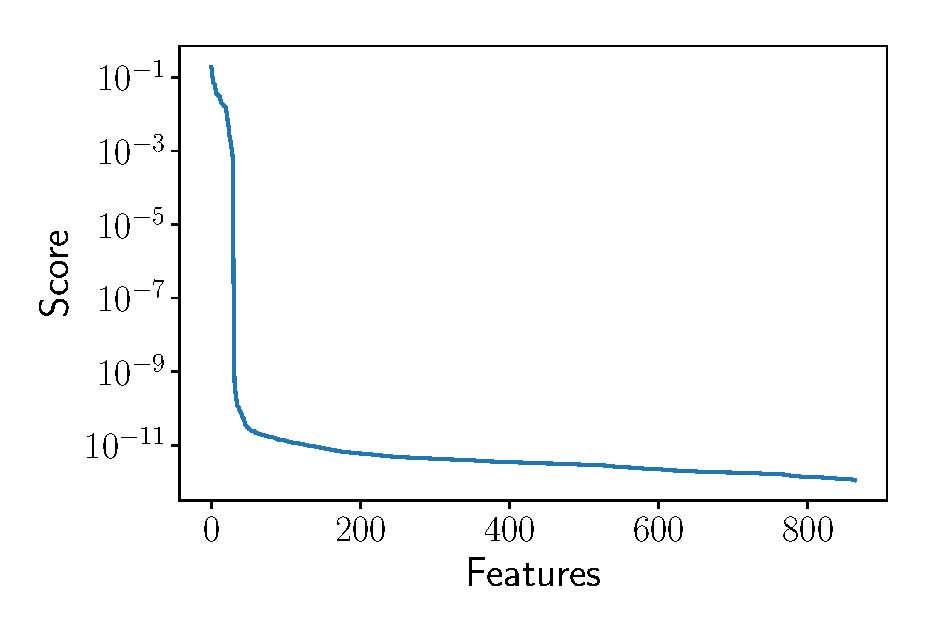
\includegraphics[width=\linewidth]{figs/feature_scores_ex.eps}
		\end{minipage}%
		\begin{minipage}{.5\linewidth}
			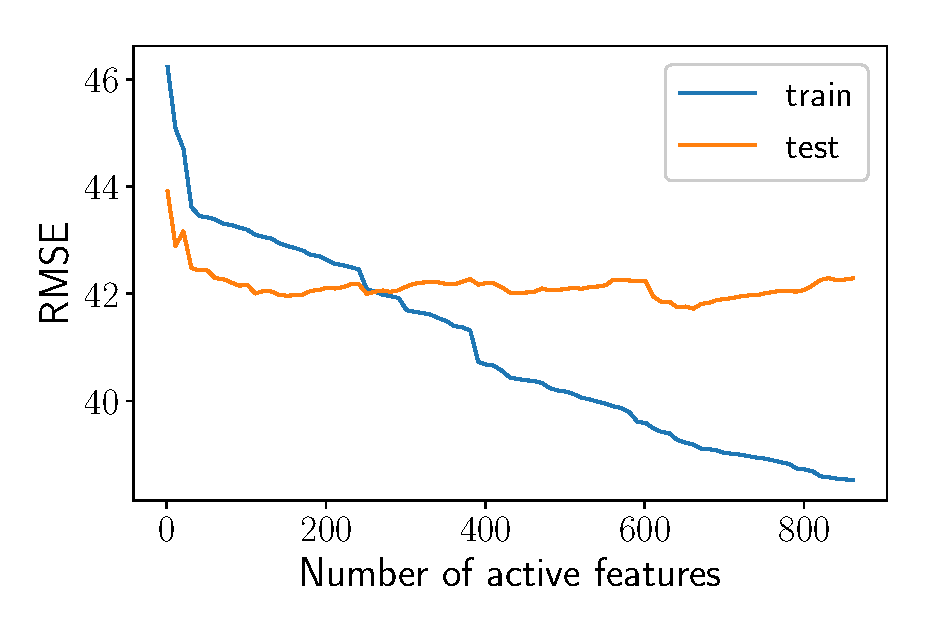
\includegraphics[width=\linewidth]{figs/train_test_qpfs.eps}
		\end{minipage}
		\centering
		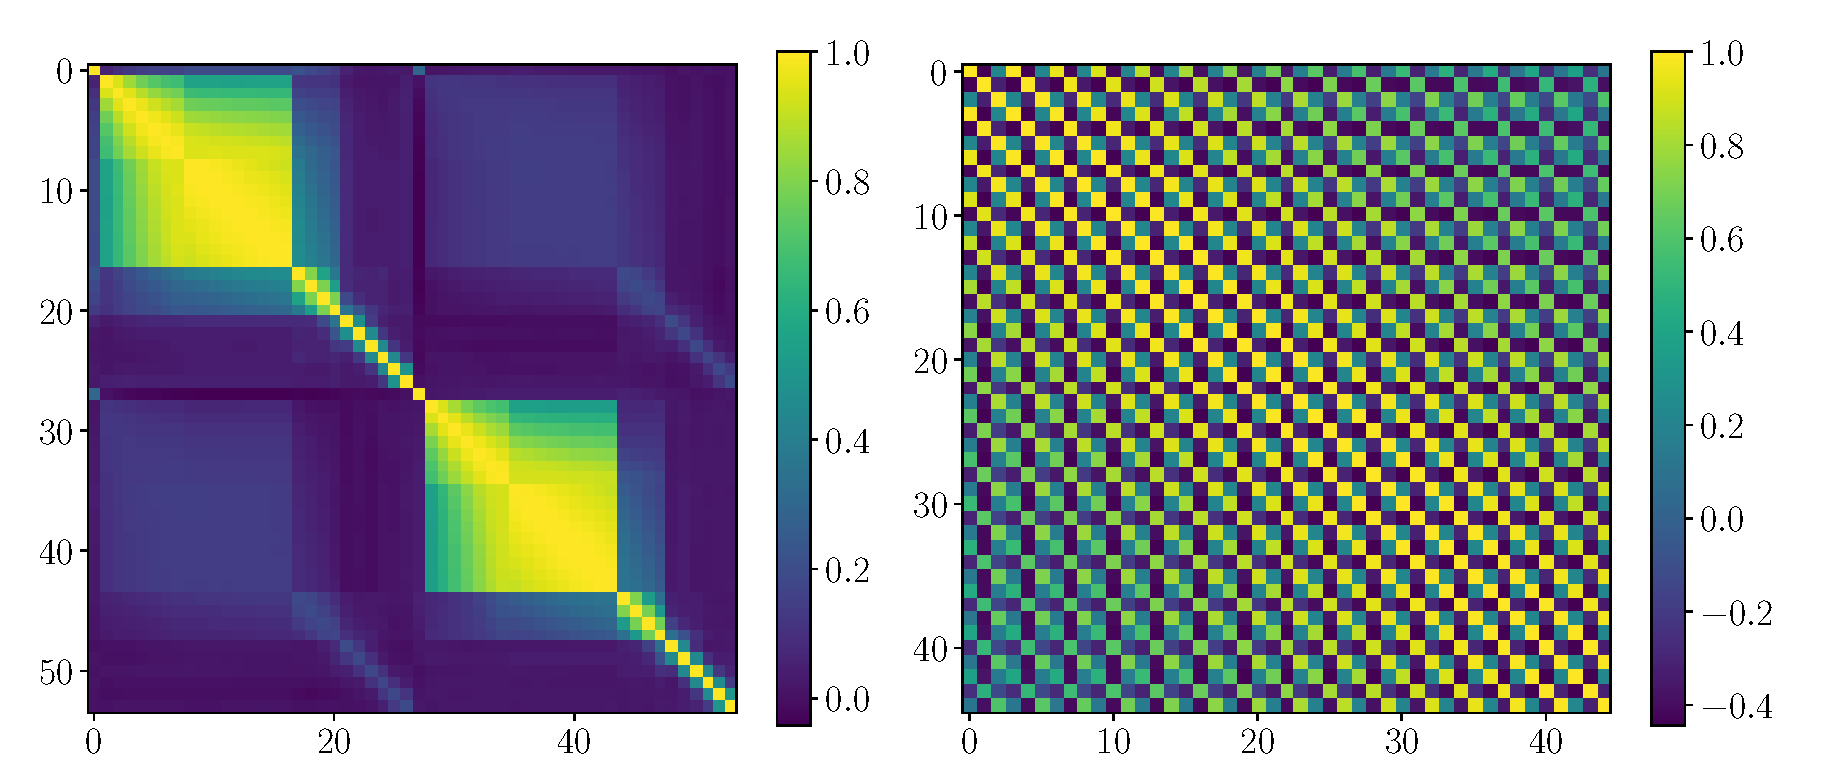
\includegraphics[width=0.9\linewidth]{figs/corr_matrix.eps}
	\end{figure}
\end{frame}
%--------------------------------------------------------------------------------
\begin{frame}{Experiment}
\begin{figure}
	\begin{minipage}{.5\linewidth}
			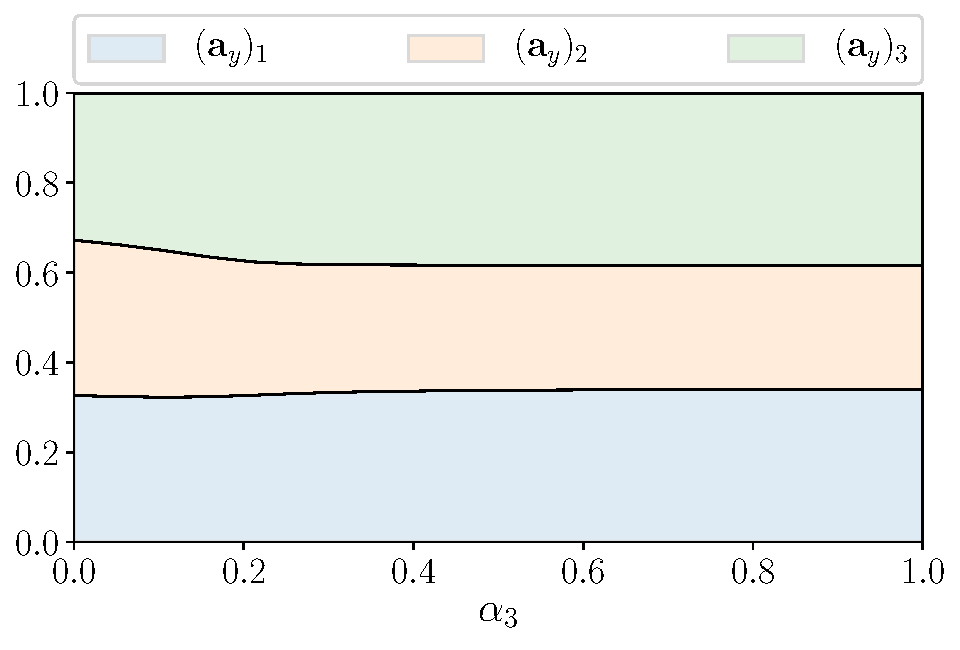
\includegraphics[width=\linewidth]{figs/features_vs_alpha_ecog_3.pdf}
	\end{minipage}%
	\begin{minipage}{.5\linewidth}
			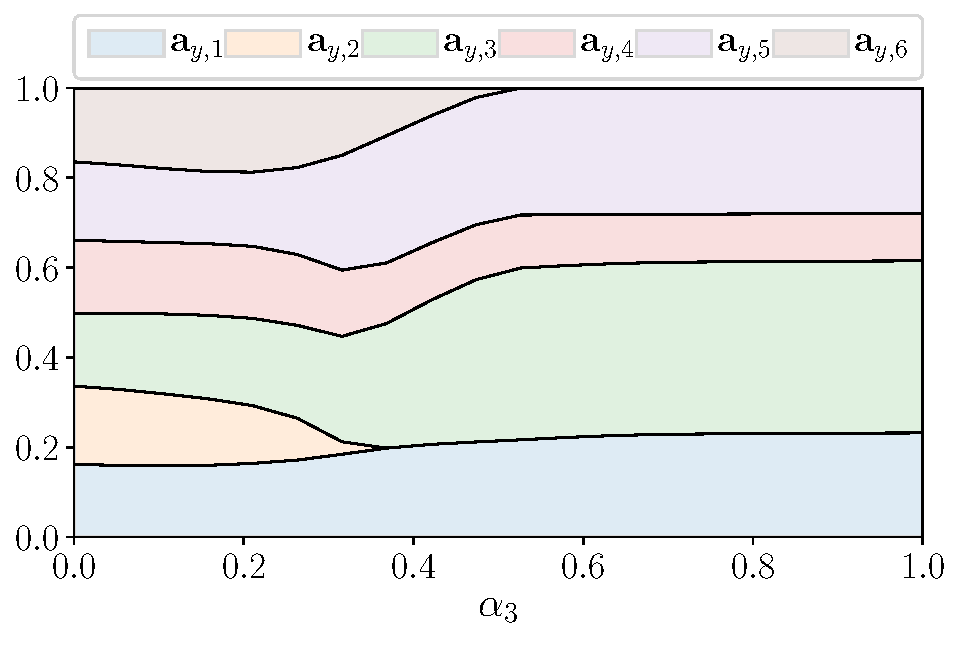
\includegraphics[width=\linewidth]{figs/features_vs_alpha_ecog_6.pdf}
	\end{minipage}\par\medskip
		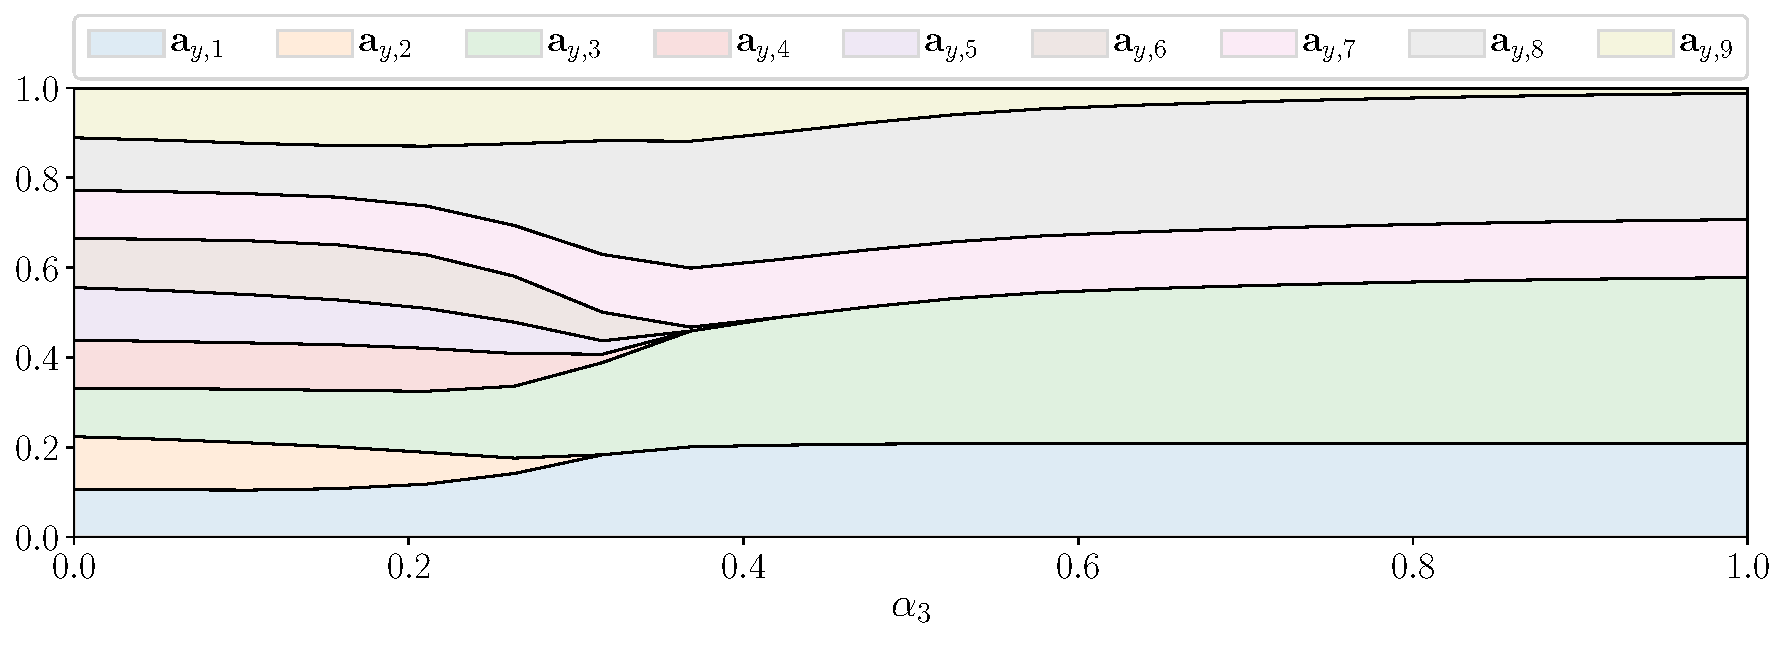
\includegraphics[width=\linewidth]{figs/features_vs_alpha_ecog_9.pdf}
\end{figure}
\end{frame}
%--------------------------------------------------------------------------------
\begin{frame}{Autoregression step = 1}
	\begin{figure}
		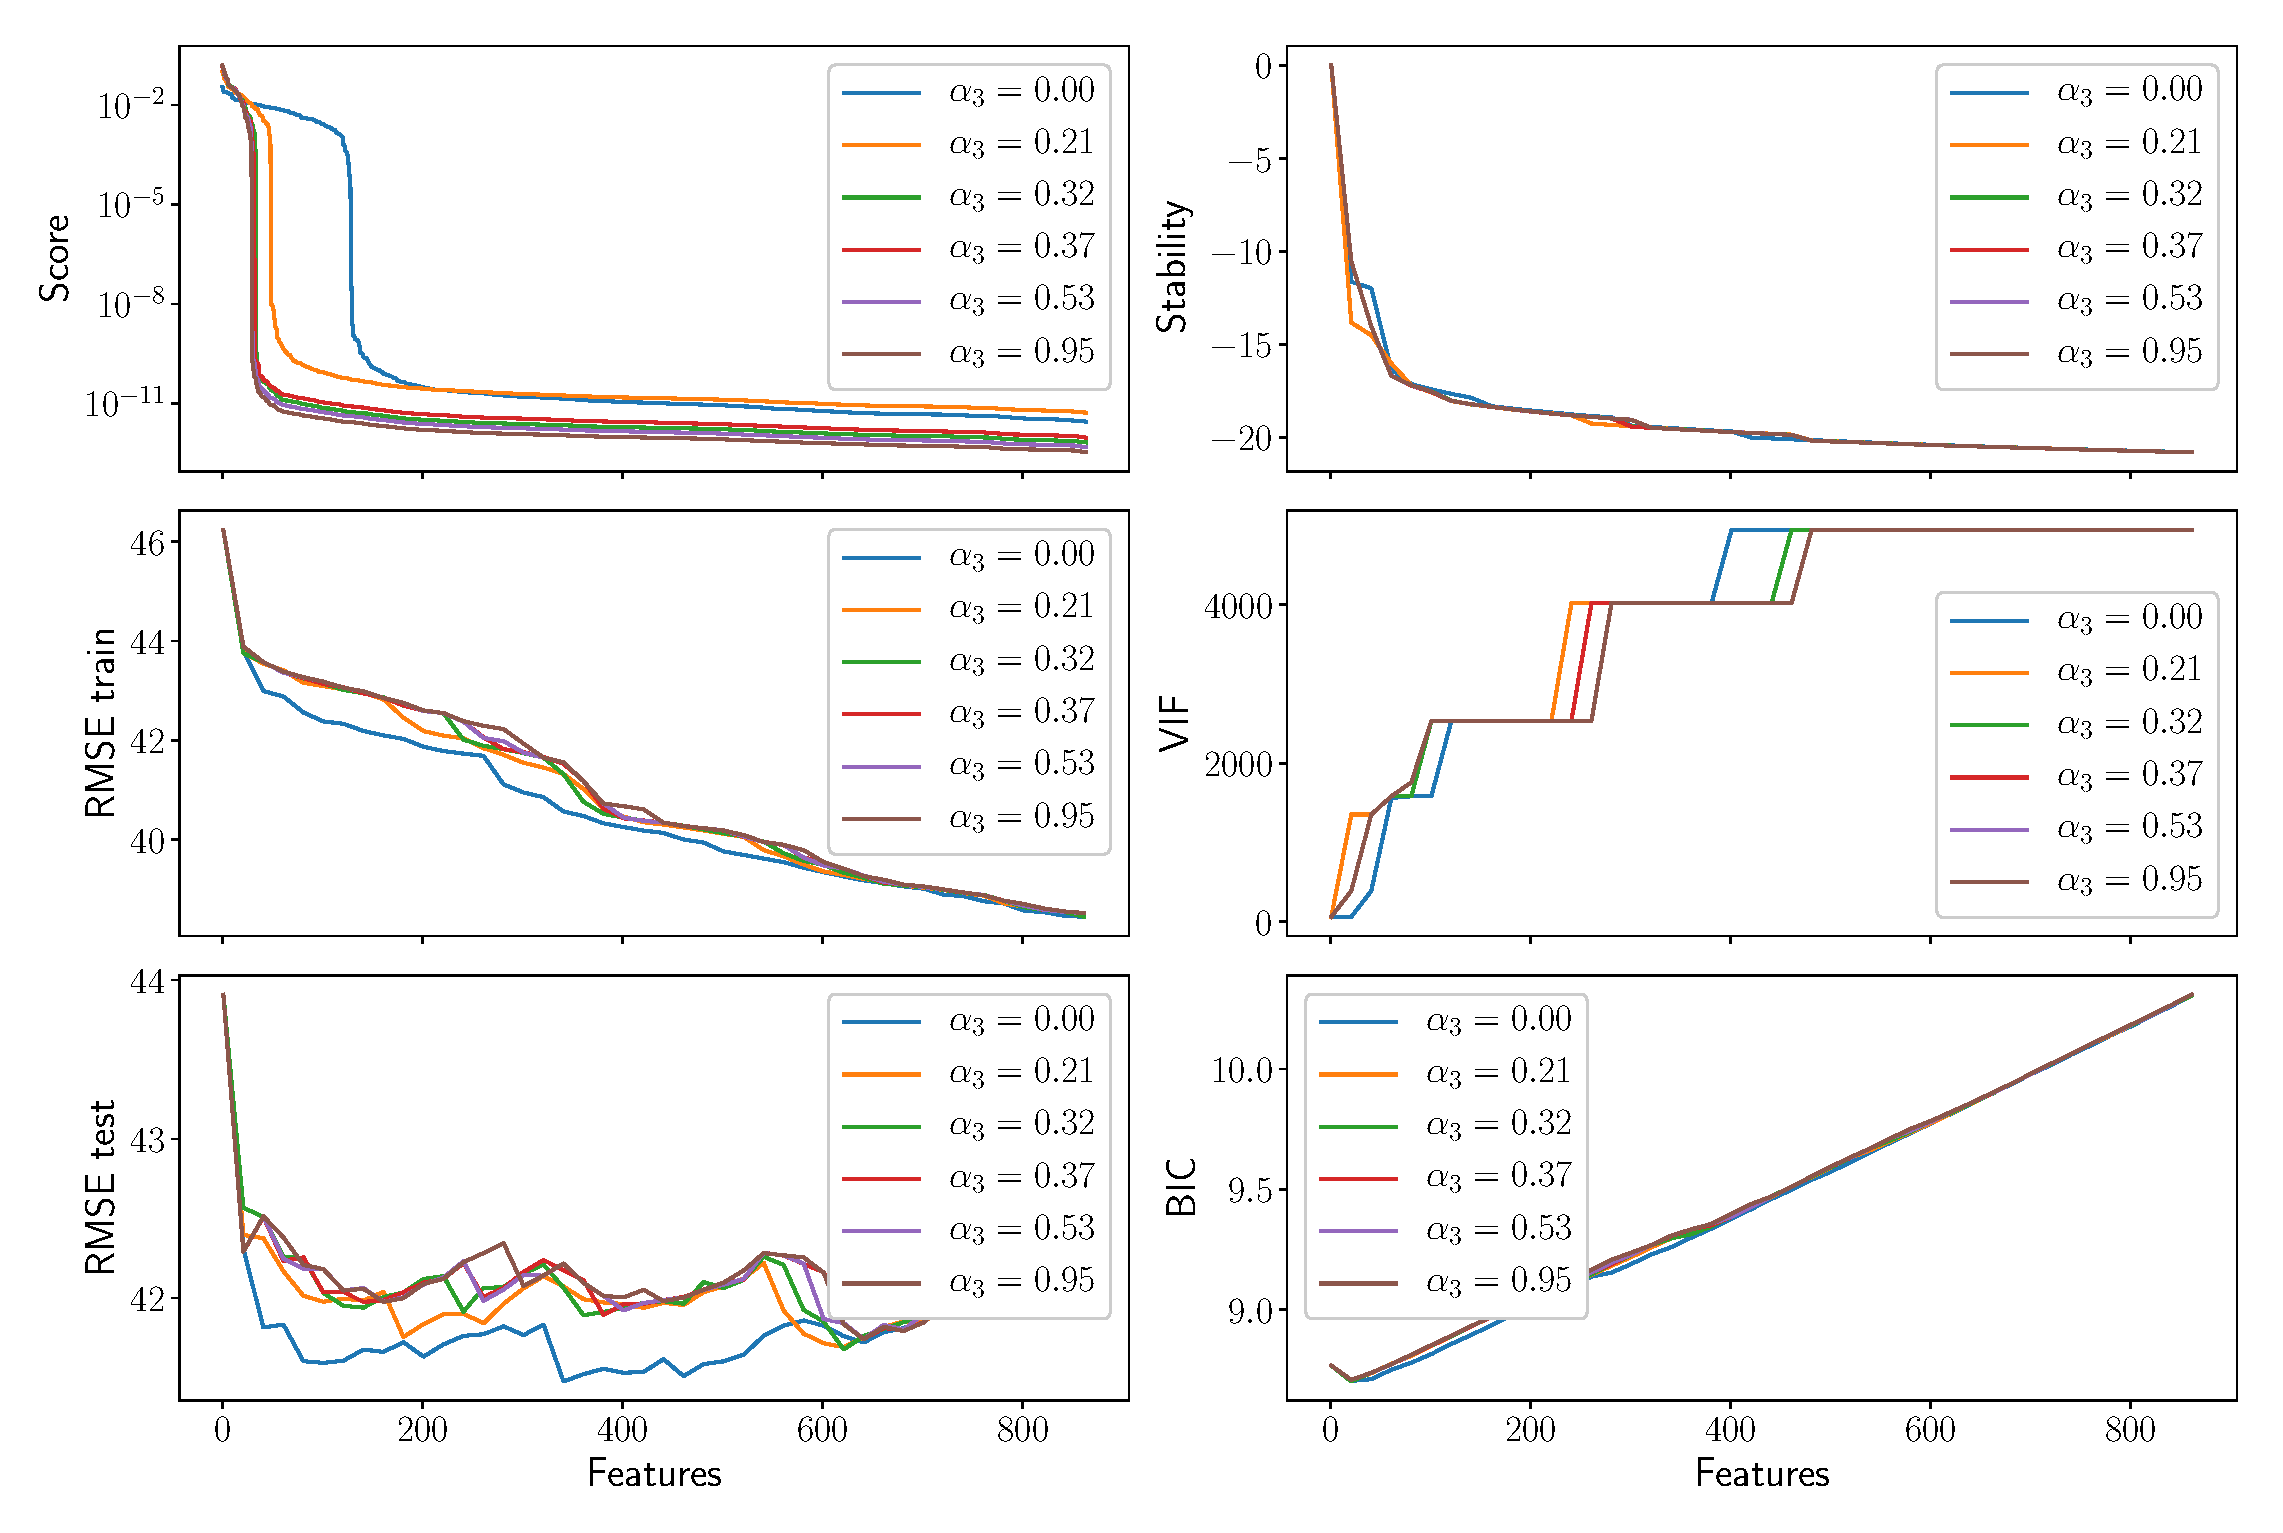
\includegraphics[width=\linewidth]{figs/ecog_3_metrics.eps}
	\end{figure}
\end{frame}

%--------------------------------------------------------------------------------
\begin{frame}{Autoregression step = 3}
	\begin{figure}
		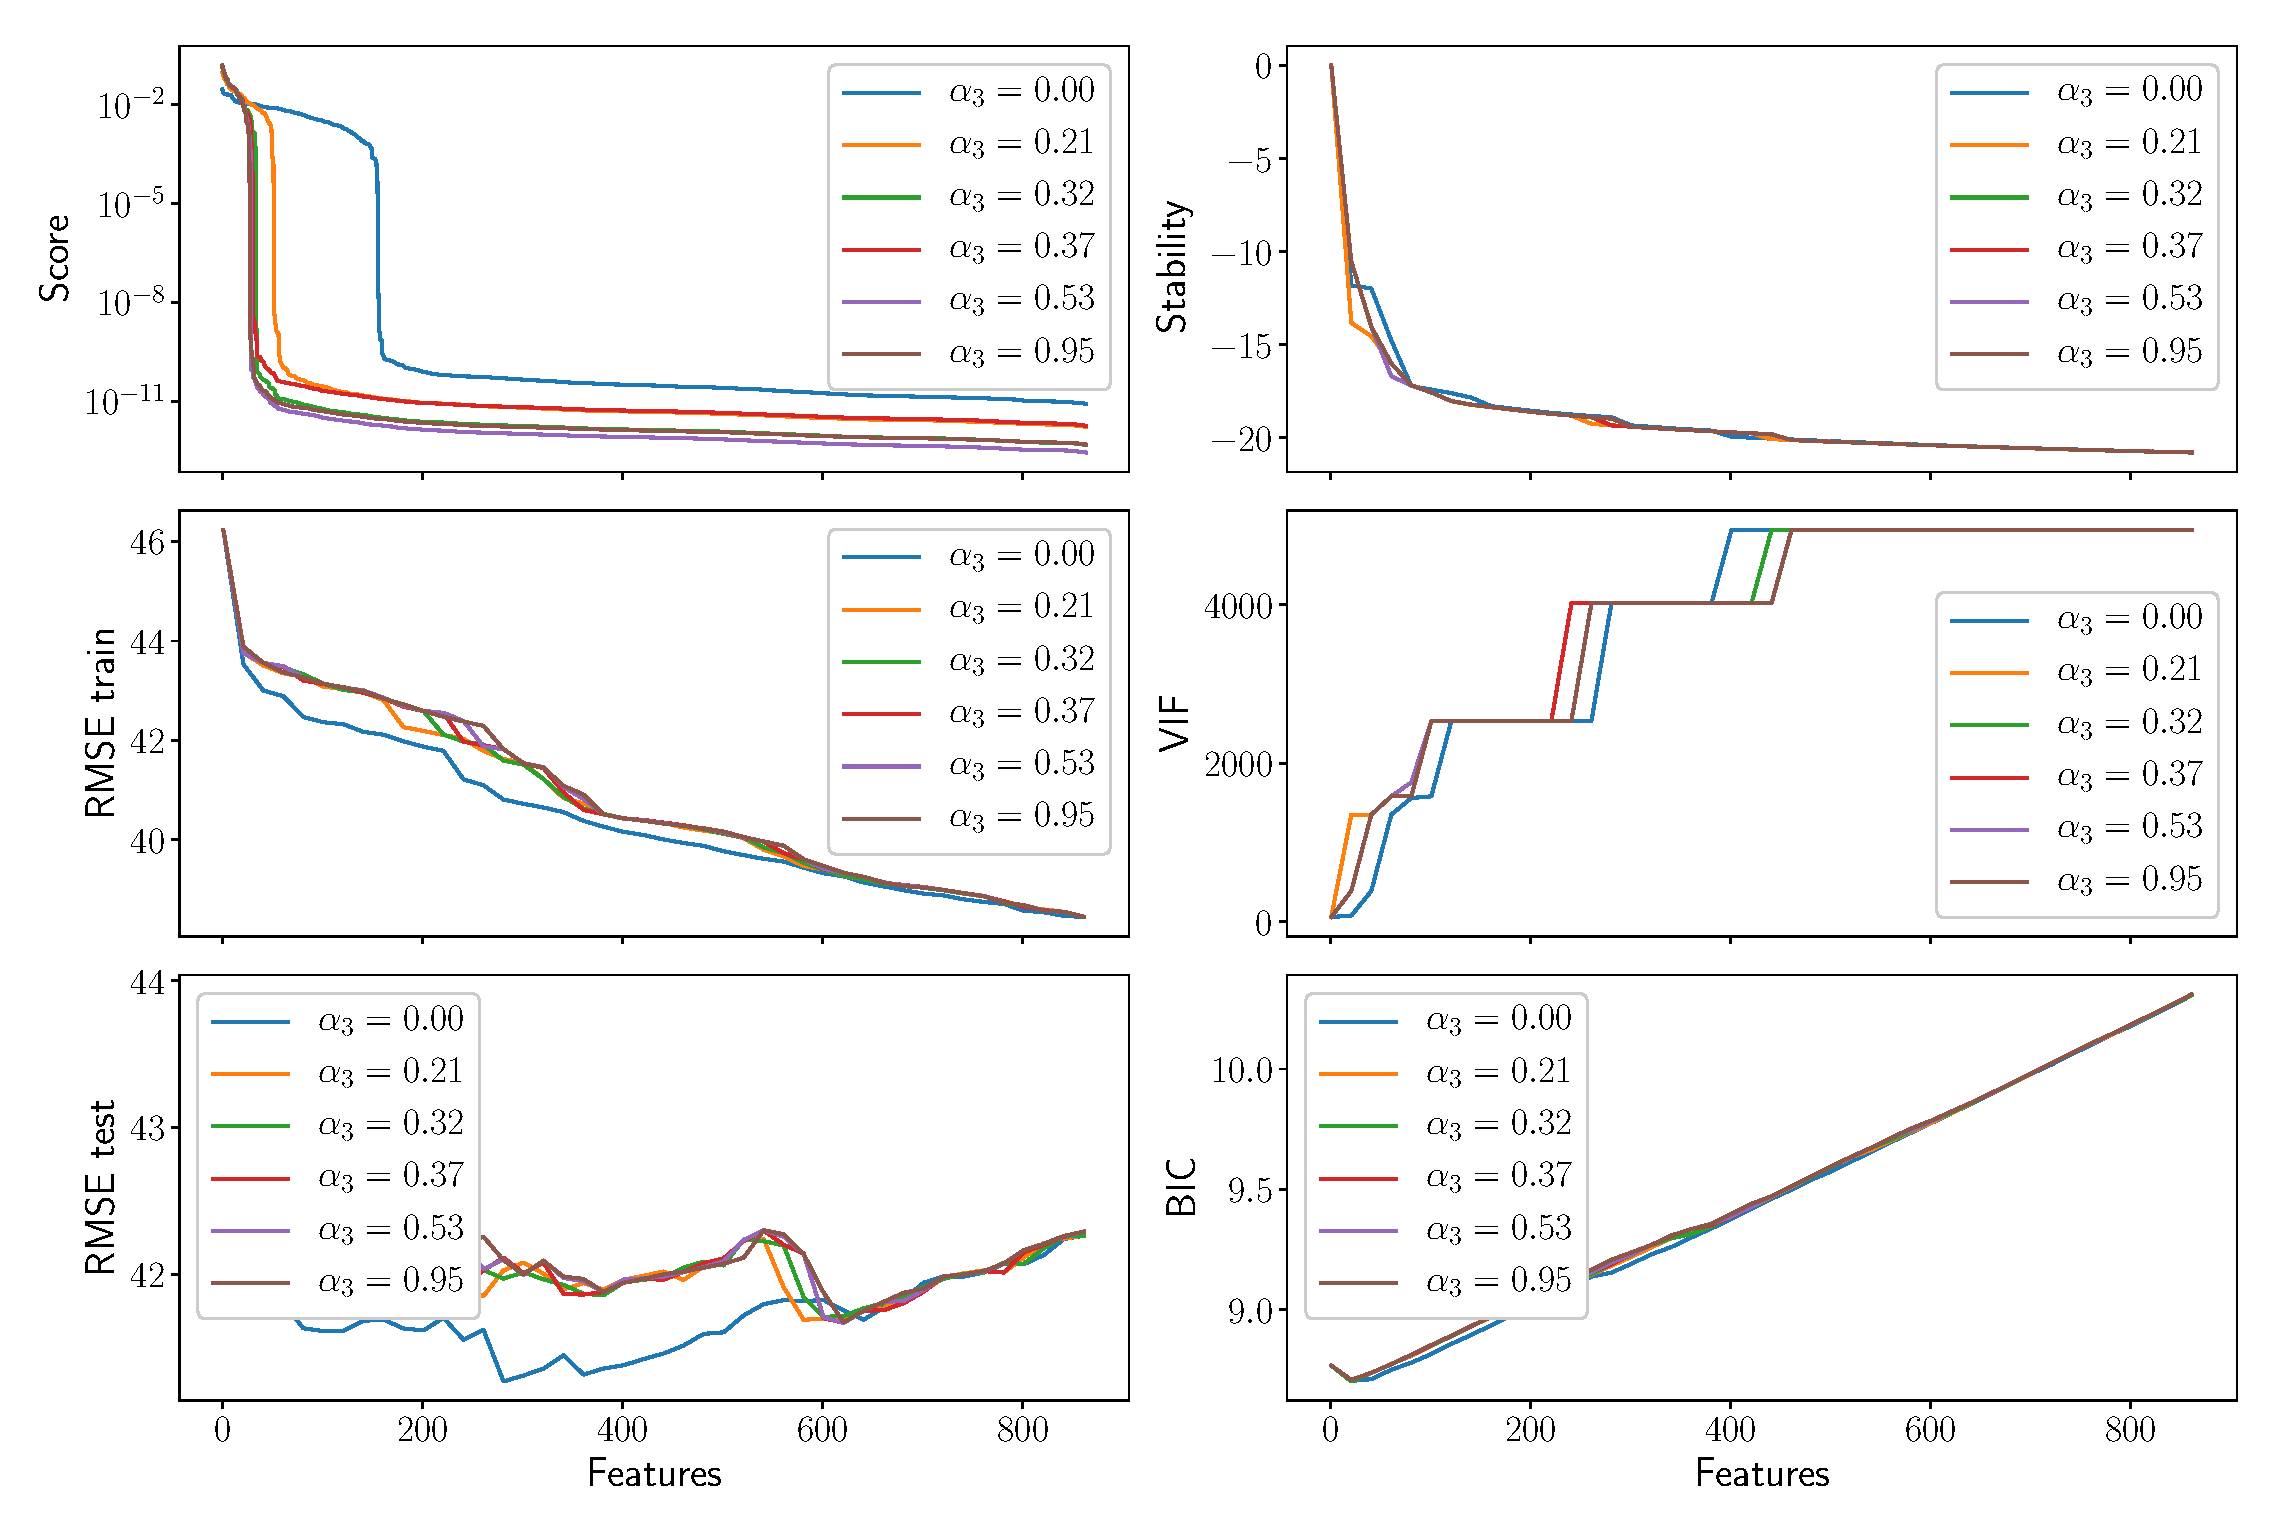
\includegraphics[width=\linewidth]{figs/ecog_9_metrics.eps}
	\end{figure}
\end{frame}
%--------------------------------------------------------------------------------
\begin{frame}{Autoregression step = 30}
	\begin{figure}
		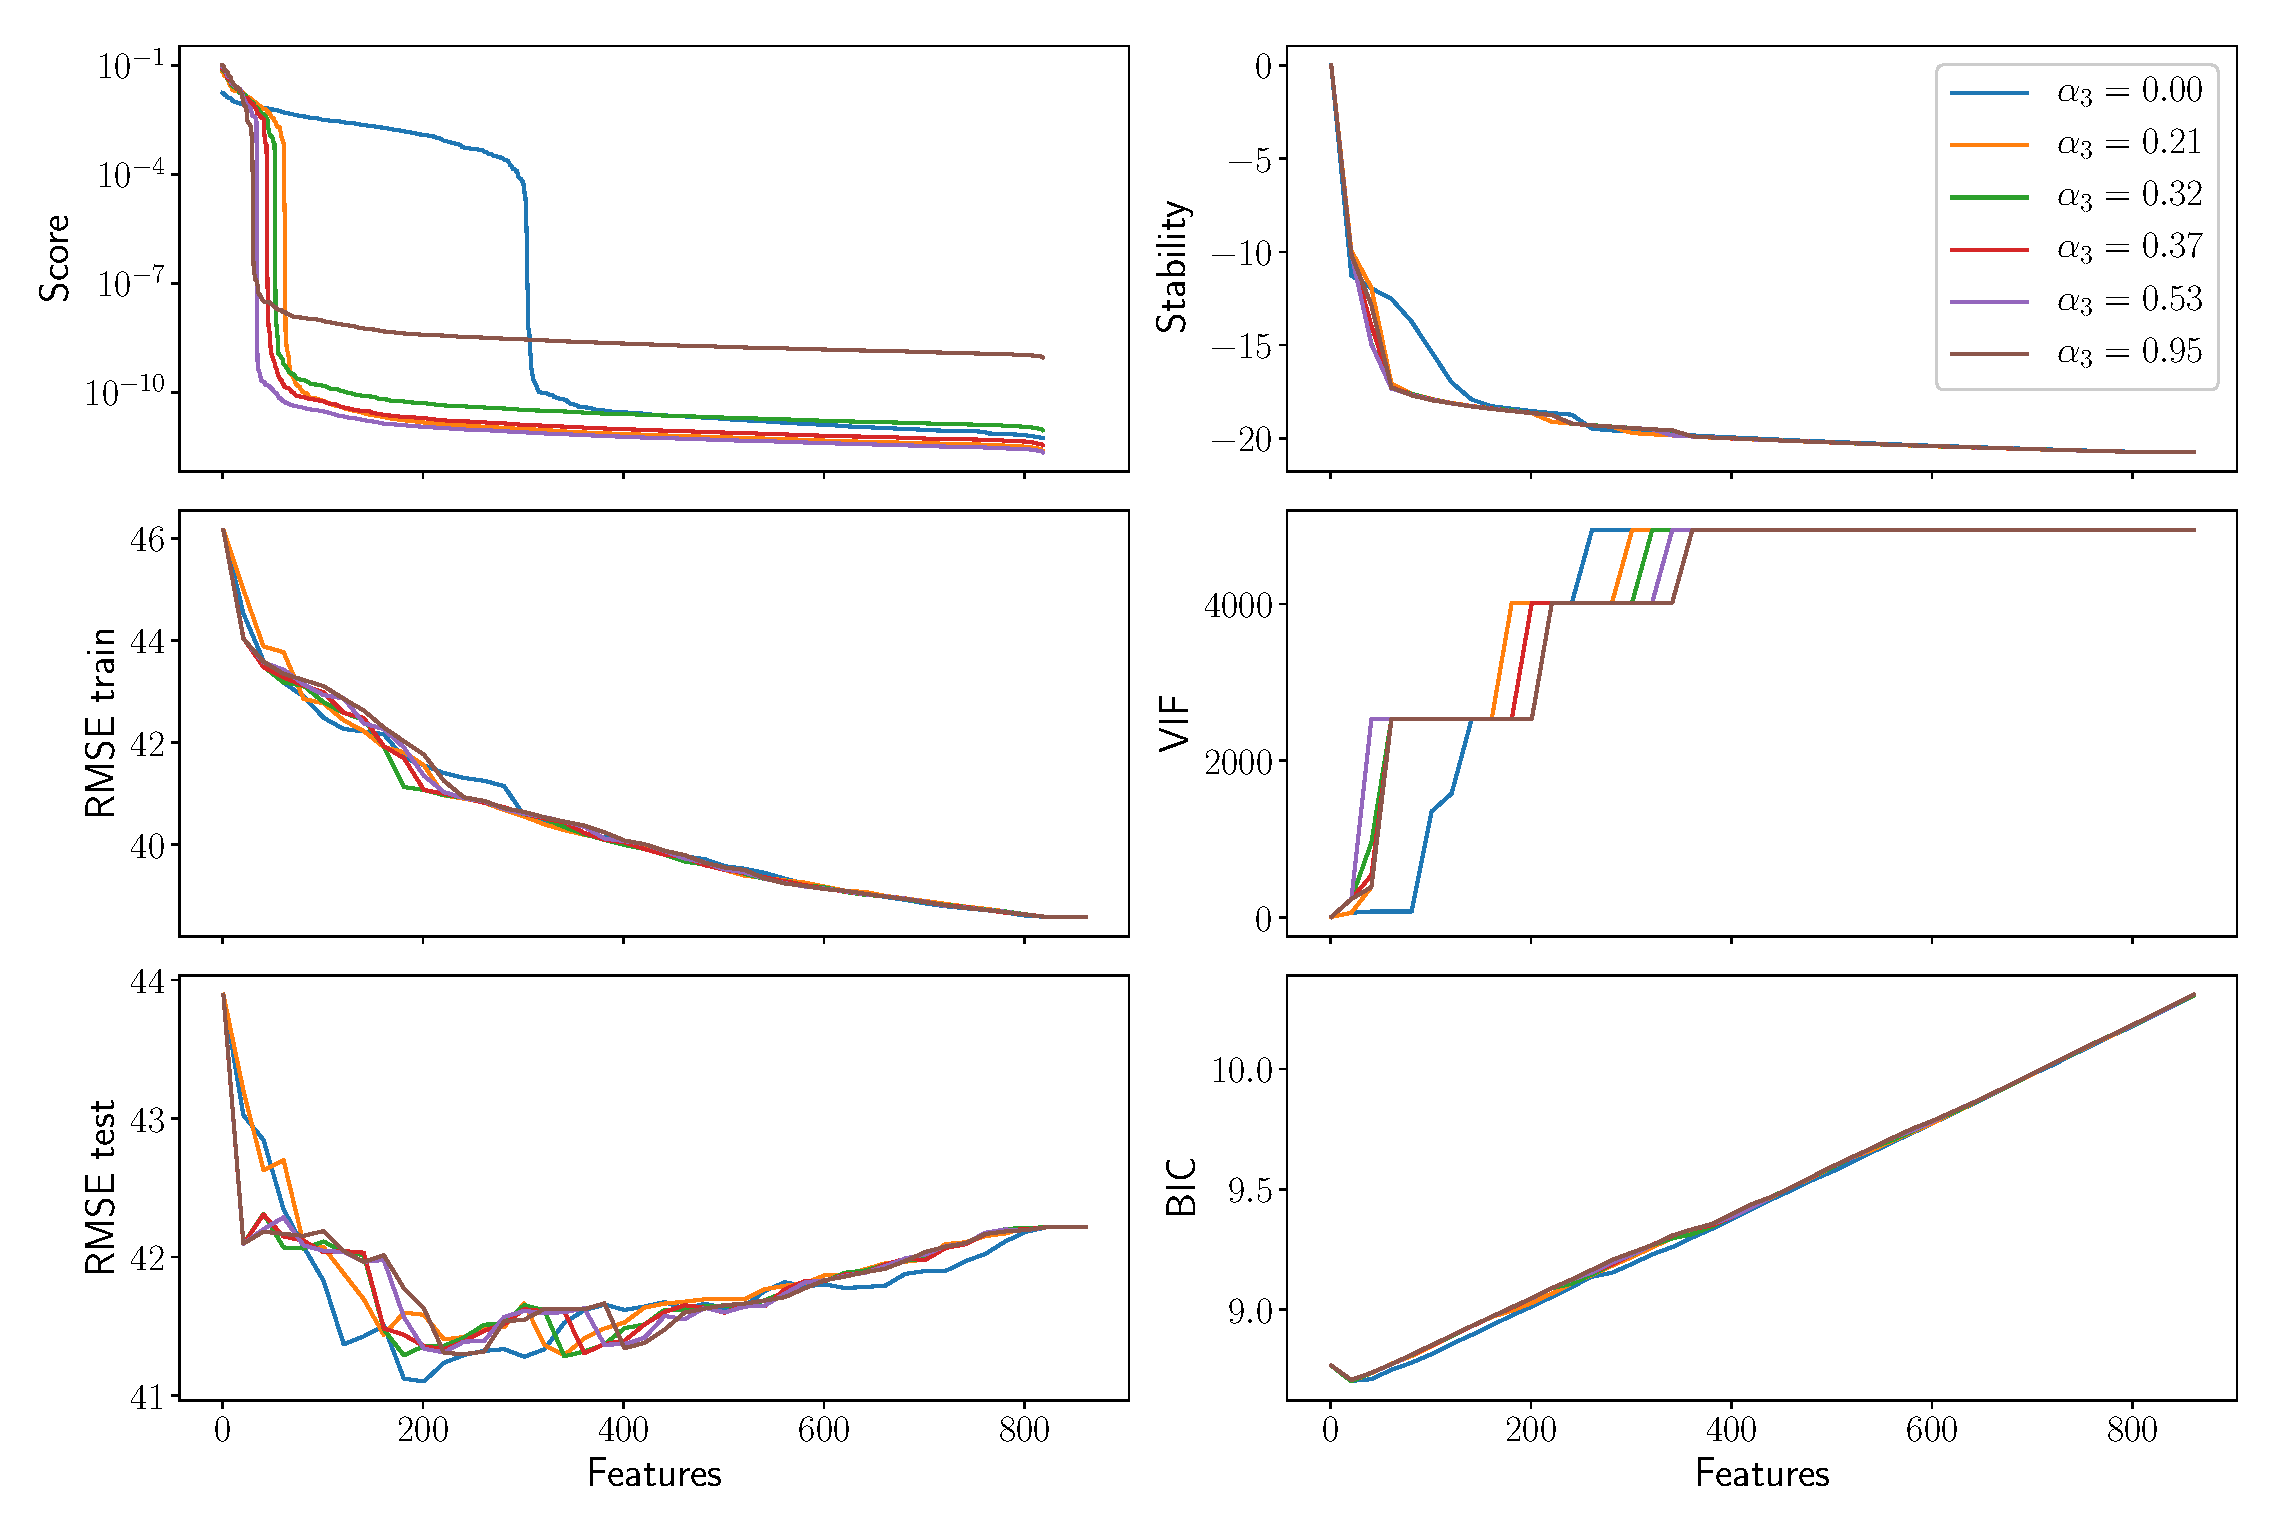
\includegraphics[width=\linewidth]{figs/ecog_90_metrics.eps}
	\end{figure}
\end{frame}
%--------------------------------------------------------------------------------
\begin{frame}{}
\end{frame}
%--------------------------------------------------------------------------------
\begin{frame}{Experiment}
\begin{figure}
	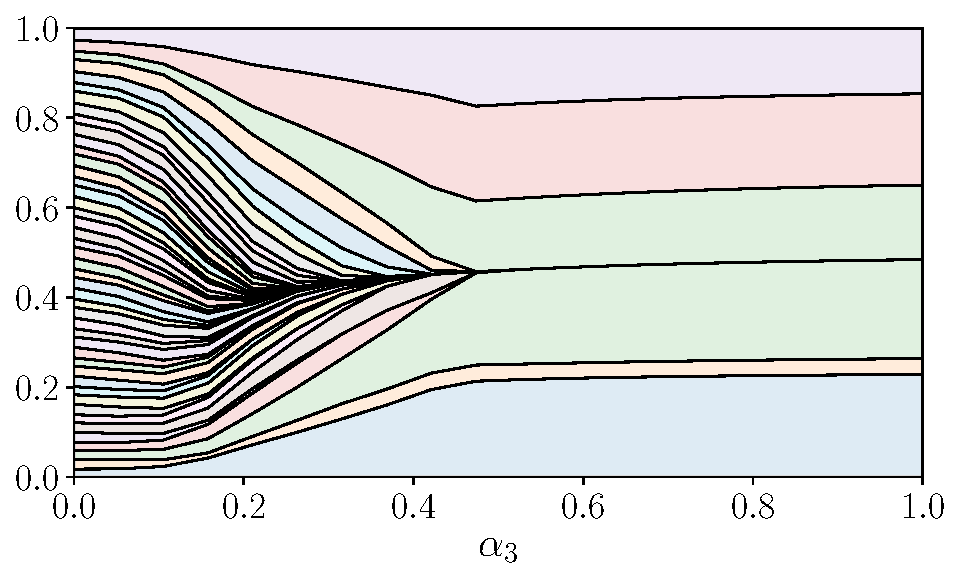
\includegraphics[width=\linewidth]{figs/features_vs_alpha_ecog_45.pdf}
	\caption{autoregression step=45}
\end{figure}
\end{frame}
%--------------------------------------------------------------------------------
\begin{frame}{Problem Statement}
\begin{minipage}{0.6\linewidth}
	\begin{figure}
		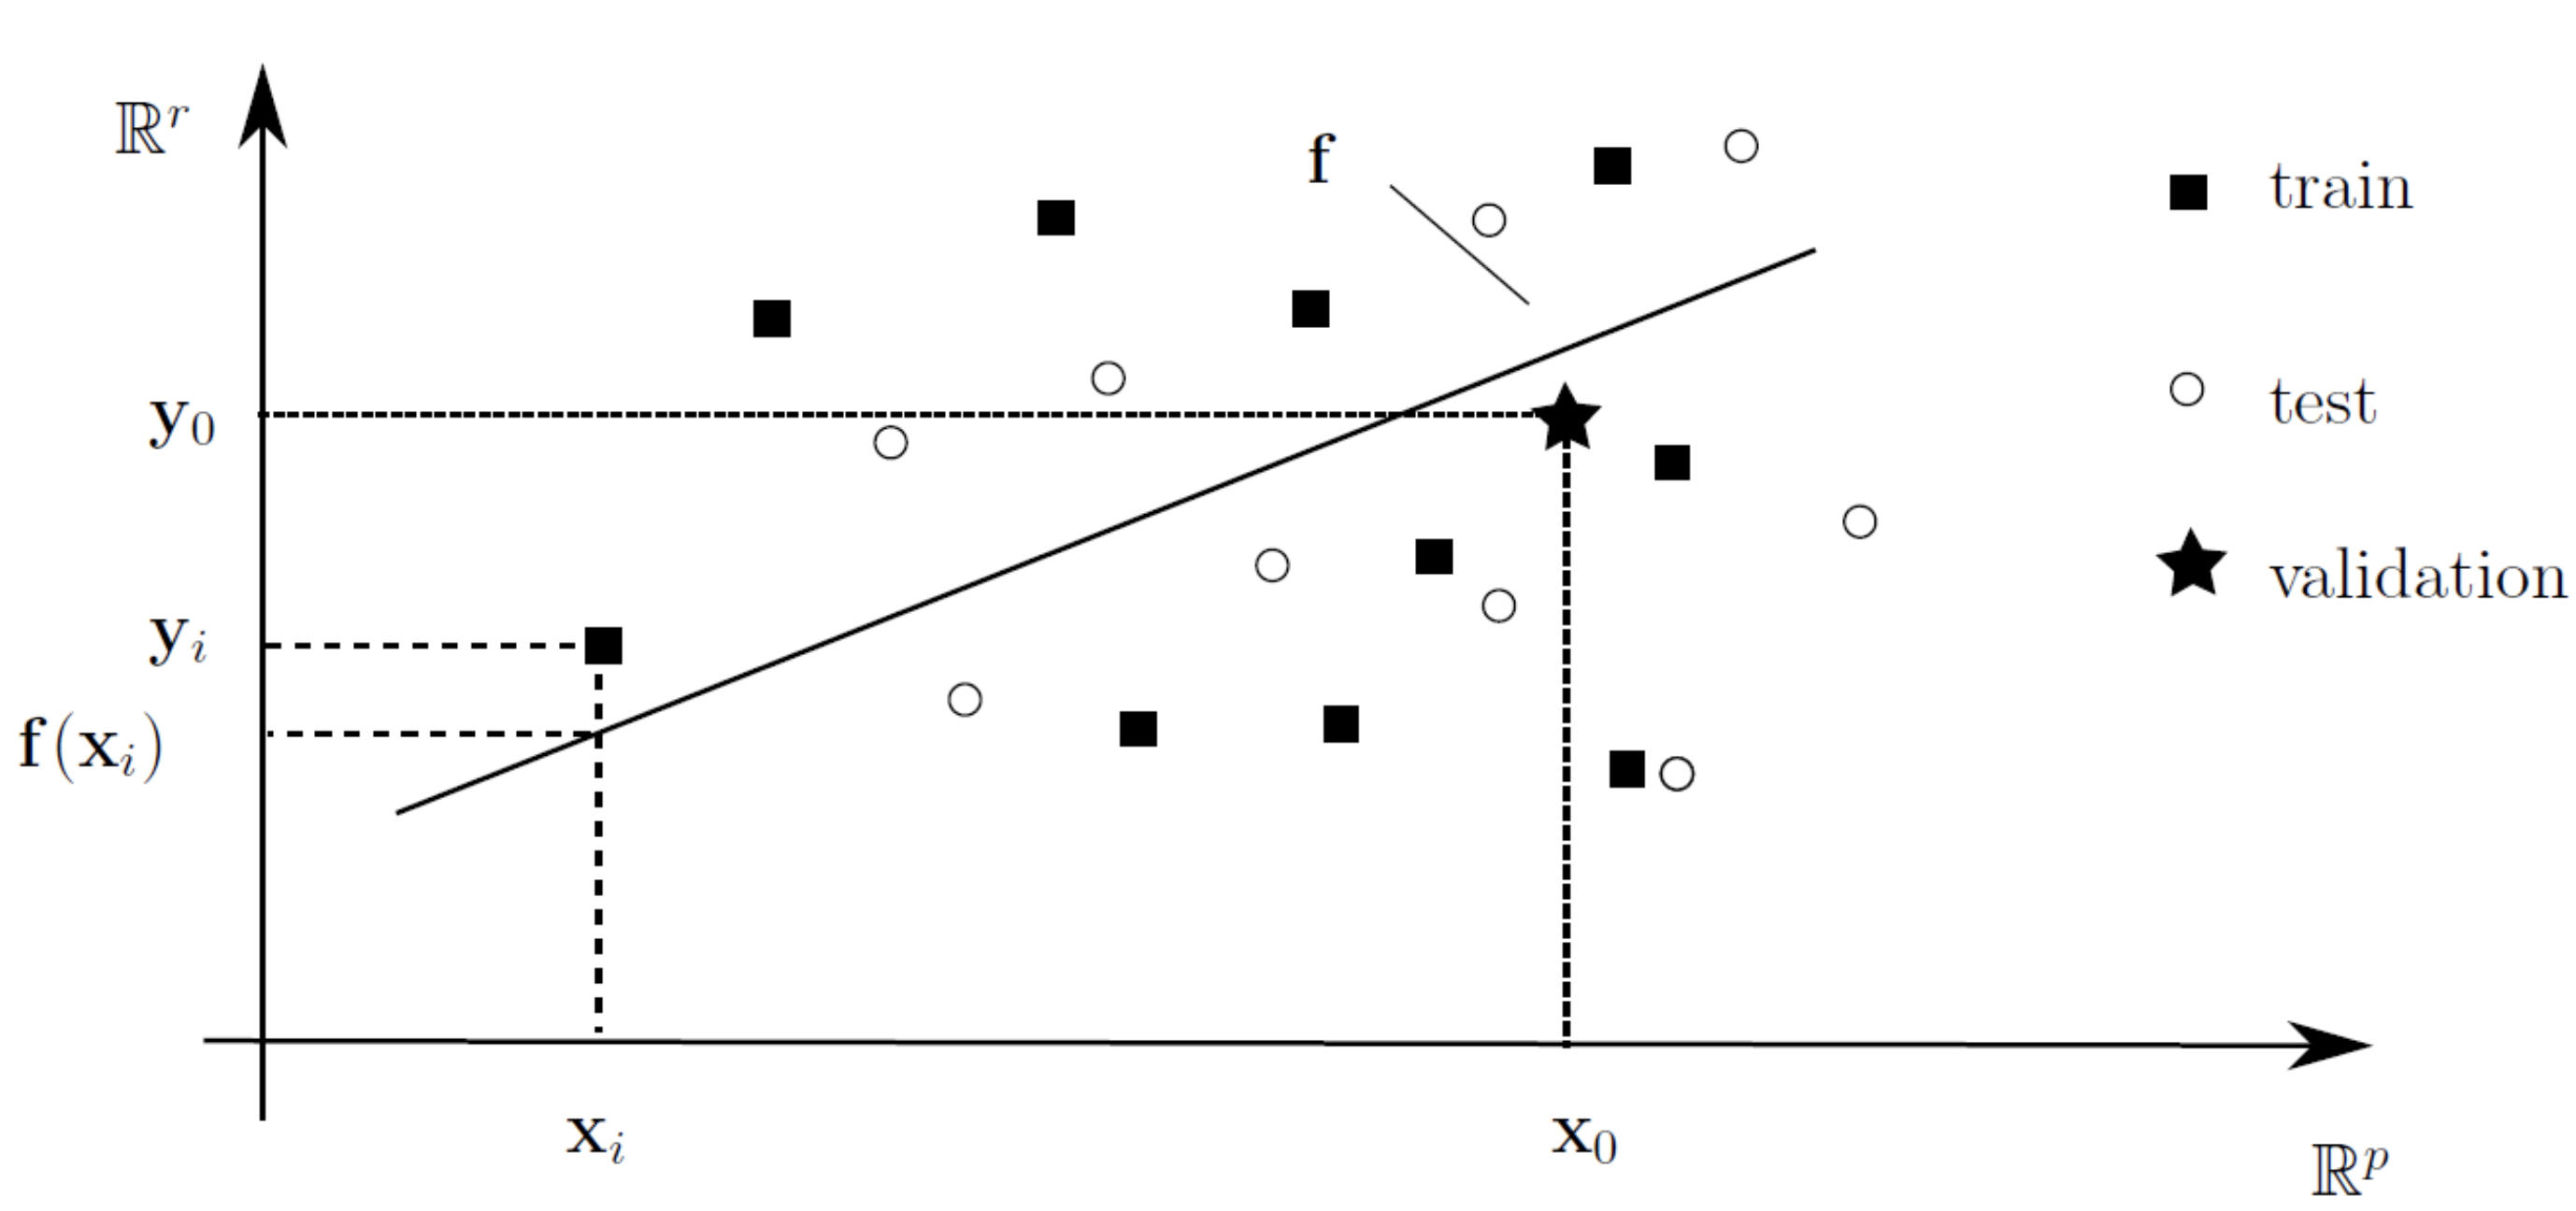
\includegraphics[width=1.1\linewidth]{figs/forecast_scheme}
	\end{figure}
	\begin{block}{Partial Least Squares (PLS)}
	\vspace{-0.5cm}
	\begin{align*}
		\underset{m \times n}{\vphantom{\bQ}\bX} 
		&= \underset{m \times l}{\vphantom{\bQ}\bT} \cdot \underset{l \times n}{\vphantom{\bQ}\bP^{T}} + \underset{m \times n}{\vphantom{\bQ}\bF} 
		= \sum_{k=1}^l \underset{m \times 1}{\vphantom{\bp_k^{T}}\bt_k} \cdot \underset{1 \times n}{\bp_k^{T}} + \underset{m \times n}{\vphantom{\bp_k^{T}}\bF}\\
		\underset{m \times r}{\vphantom{\bQ}\bY} 
		&= \underset{m \times l}{\vphantom{\bQ}\bU} \cdot \underset{l \times r}{\bQ^{T}} + \underset{m \times r}{\vphantom{\bQ}\bE}
		=  \sum_{k=1}^l  \underset{m \times 1}{\vphantom{\bq_k^{T}}\bt_k} \cdot \underset{1 \times r}{\bq_k^{T}} +  \underset{m \times r}{\vphantom{\bq_k^{T}}\bE}
	\end{align*}
	\end{block}
	\begin{equation*}
		\mathbf{\hat{Y}} = \mathbf{T}\text{diag}(\boldsymbol{\beta}) \bQ^{T} = \bX \bTheta.
	\end{equation*}
\end{minipage}%
\begin{minipage}{0.4\linewidth}
	
	\begin{figure}
		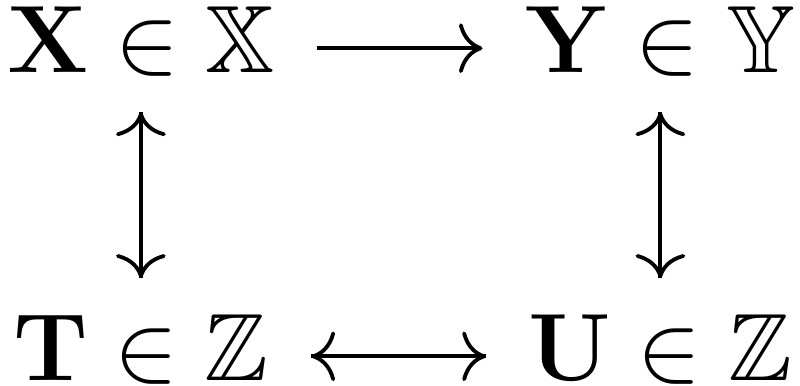
\includegraphics[width=0.6\linewidth]{figs/diagram}
	\end{figure}
	\vspace{1cm}
	\begin{itemize}
		\item map $\bX$ into low-dimensional~$\bT$;
		\item map $\bY$ into low-dimensional~$\bU$;
		\item maximize correlation between $\bt_k$ and $\bu_k$.
	\end{itemize}
\end{minipage}
\end{frame}
%--------------------------------------------------------------------------------
\begin{frame}{PLS Example}
	\begin{figure}
		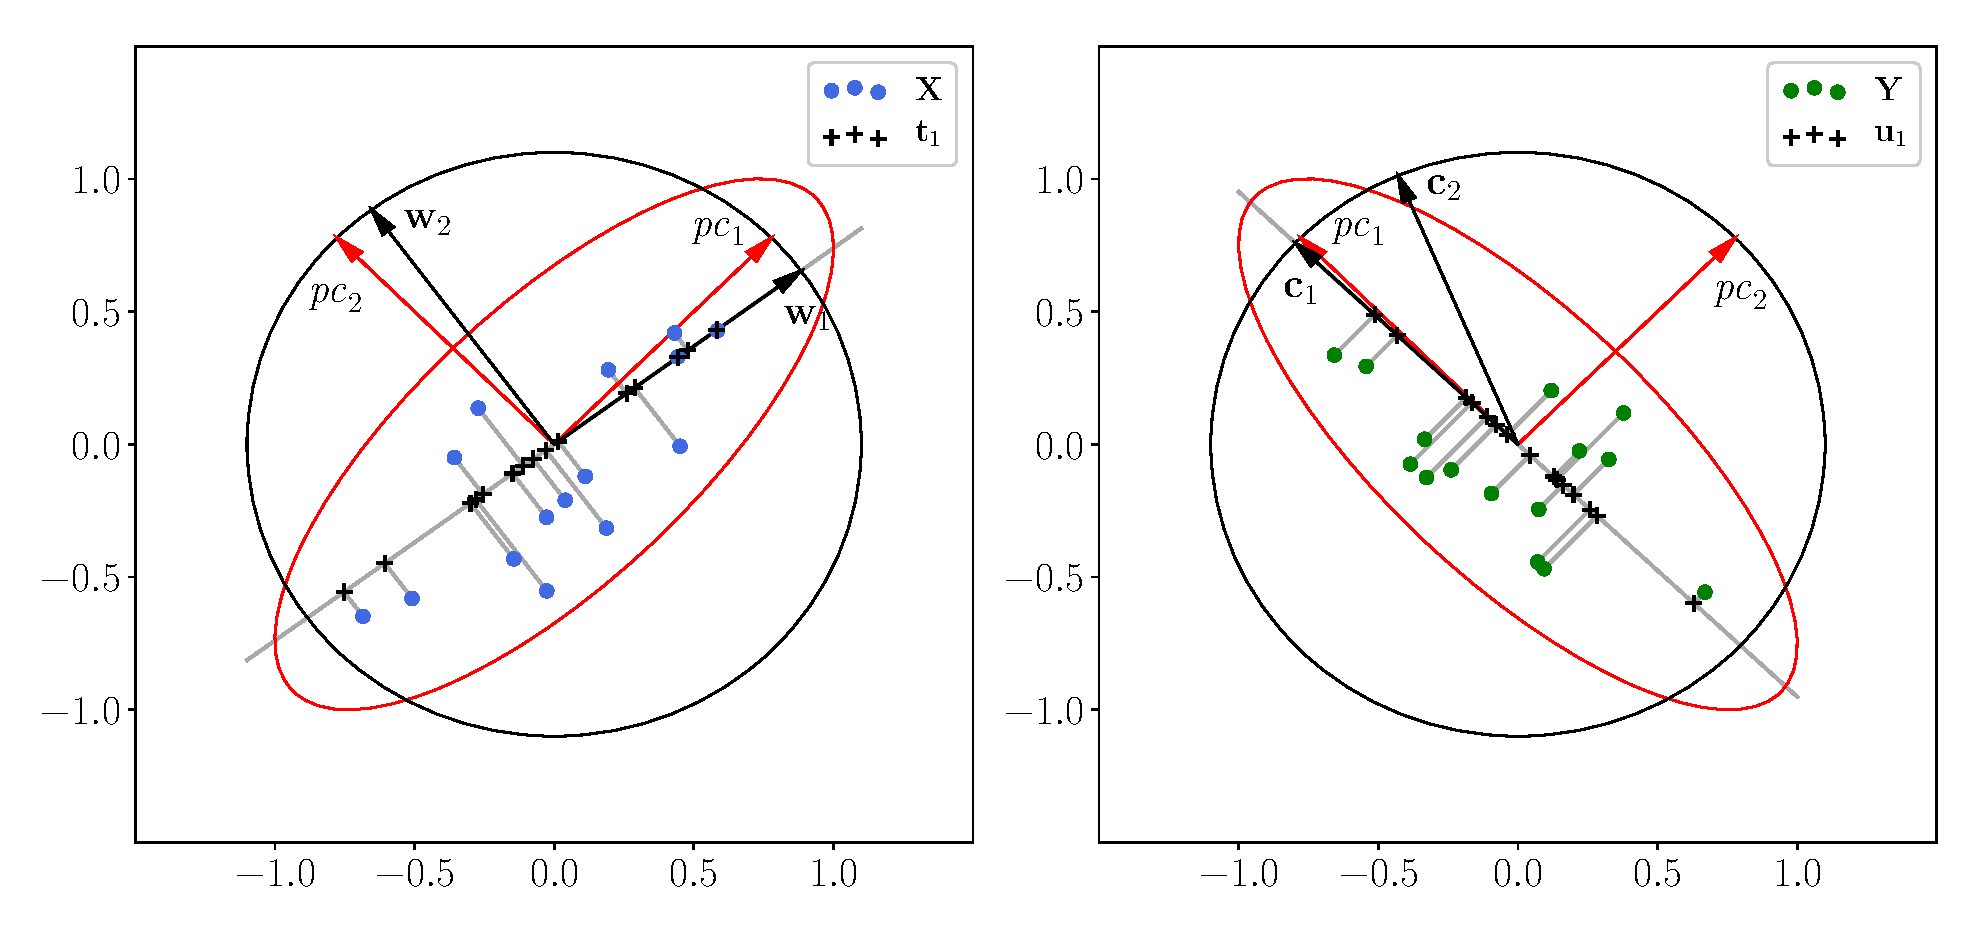
\includegraphics[width=\linewidth]{figs/PLSFigure.eps}
		\caption{The result of the PLS algorithm for the case $n = r = l = 2$.}
	\end{figure}
\end{frame}
%--------------------------------------------------------------------------------
\begin{frame}{Computational experiment}
	\begin{minipage}{0.55\textwidth}
		\begin{block}{Datasets}
			\vspace{0.35cm}
			\begin{itemize}
				\item energy consumption
				\item electrocorticogram signals (ECoG)
			\end{itemize}
		\end{block}
		\vspace{0.5cm}
	\end{minipage}%
	\begin{minipage}{0.45\textwidth}
		\begin{block}{Autoregressive approach}
				\[
				\mathbf{X} = 
				\begin{pmatrix}
				x_1 & x_2 & \dots & x_n \\
				x_2 & x_3 & \dots & x_{n+1} \\
				\dots & \dots & \dots & \dots \\
				x_{T-n+1} & x_{T-n+2} & \dots & x_T
				\end{pmatrix}
				\]
		\end{block}
	\end{minipage}
	\begin{block}{ECoG data}
	\begin{figure}
		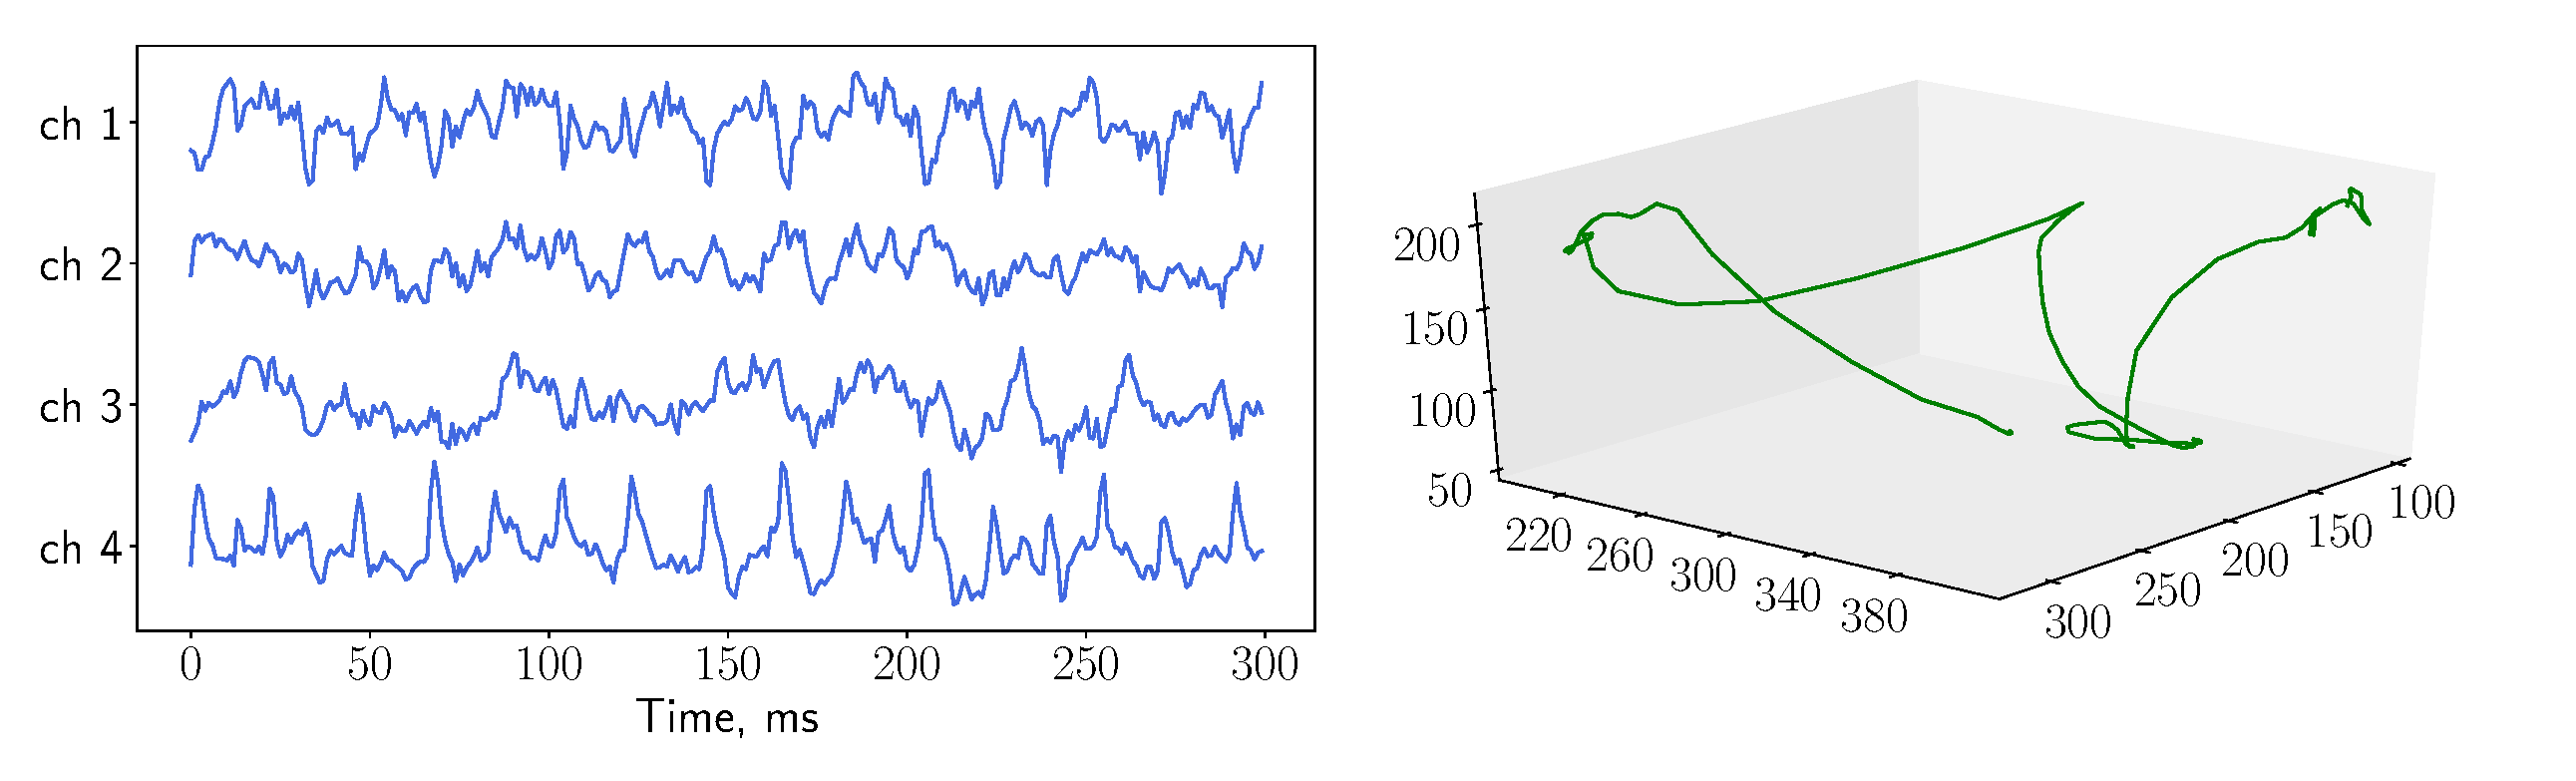
\includegraphics[width=\linewidth]{figs/ecog_data}
	\end{figure}
	\end{block}
\end{frame}
%--------------------------------------------------------------------------------
\begin{frame}{Computational experiment}
	\begin{block}{Energy consumption}
	\begin{figure}
		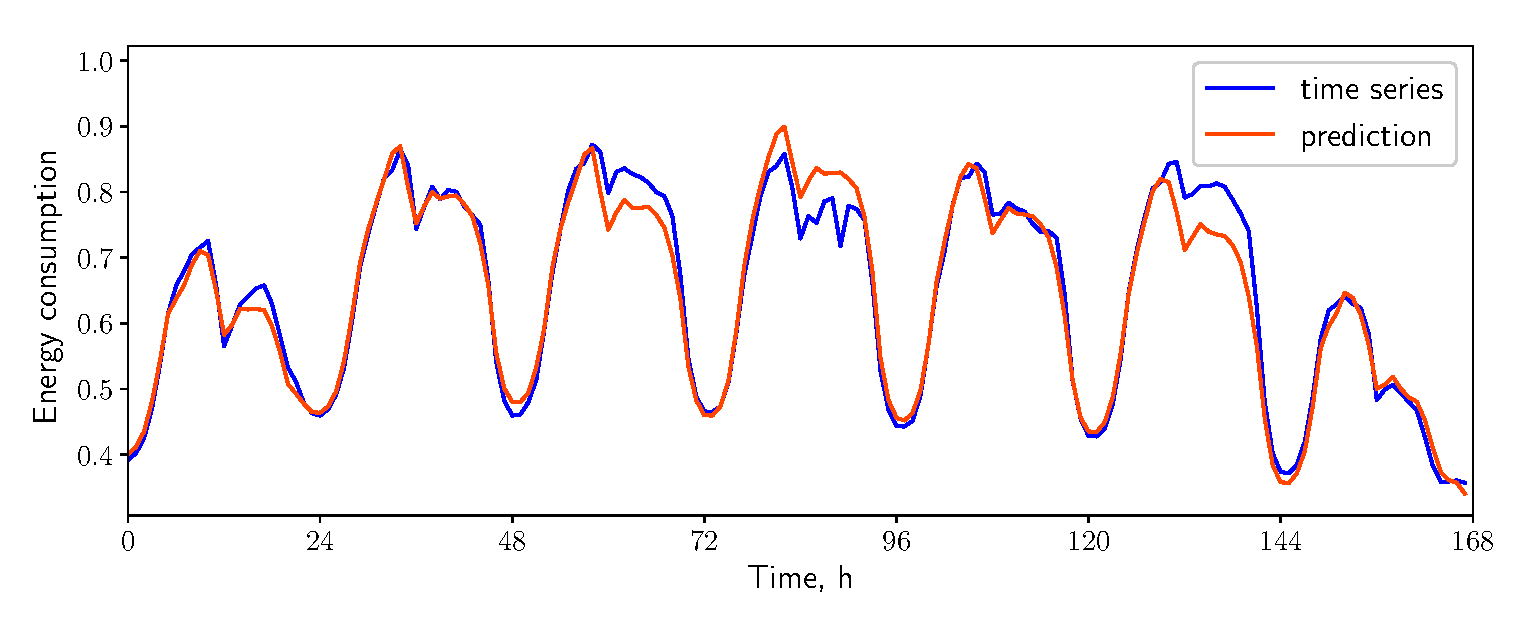
\includegraphics[width=0.8\linewidth]{figs/energy_prediction_pres.eps}
	\end{figure}
	\vspace{-0.5cm}
	\end{block}
	\begin{block}{Results}
	\begin{itemize}
		\item Space dimensionalities: $\bX = 700 \times (24 \cdot 7)$ , $\bY = 700 \times 24$.
		\item Dimensionality of latent space: 14
		\item NMSE: 0.047
	\end{itemize}
	\end{block}
\end{frame}
%--------------------------------------------------------------------------------
\begin{frame}{Computational experiment}
	\begin{block}{ECoG}
	\begin{figure}
		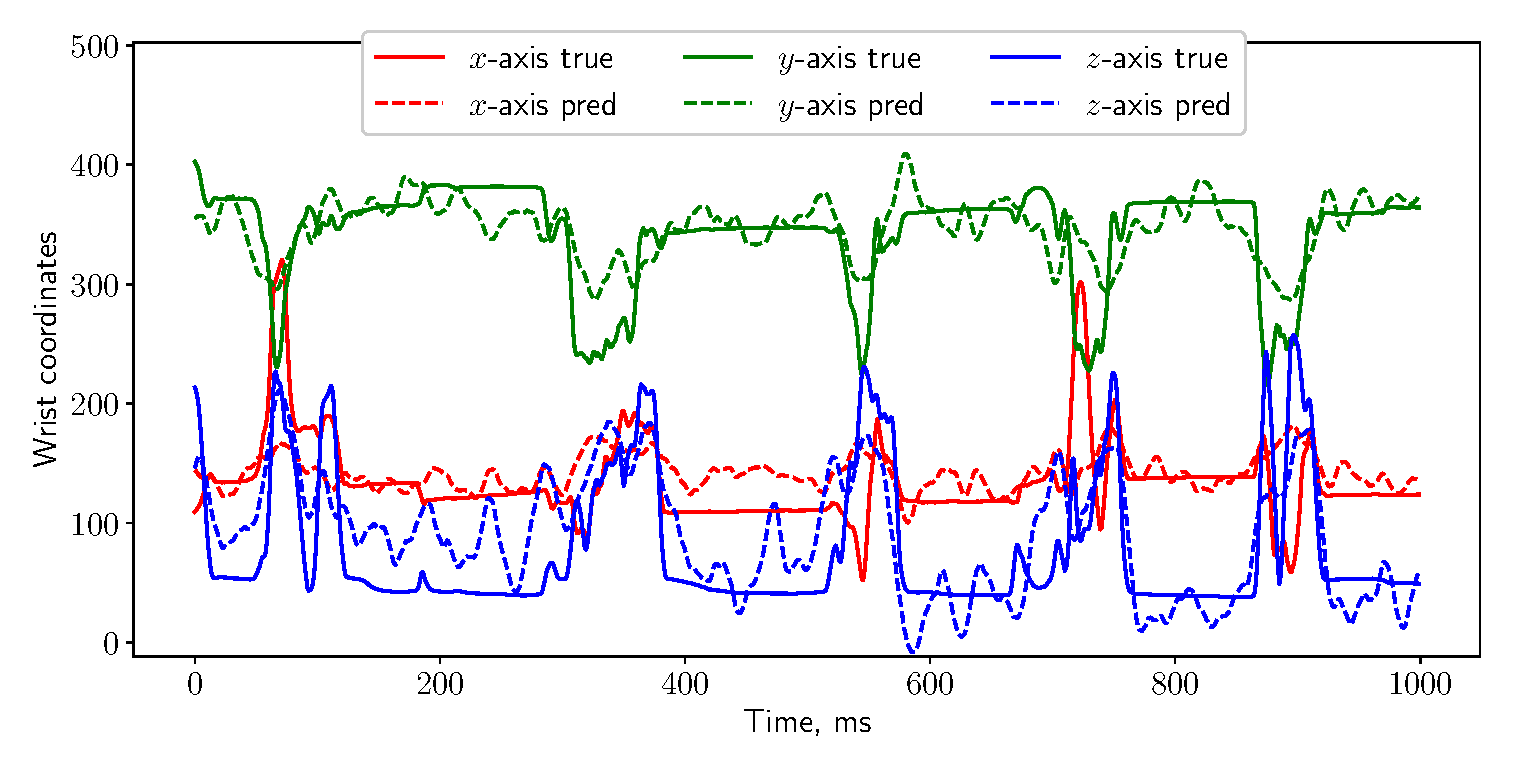
\includegraphics[width=0.8\linewidth]{figs/ecog_prediction_pres.eps}
	\end{figure}
	\end{block}
	\begin{block}{Results}
		\begin{itemize}
			\item Space dimensionalities: $\bX = 13000 \times (864 \cdot 18)$ , $\bY = 13000 \times 3$.
			\item Dimensionality of latent space: 16
			\item NMSE: 0.731
		\end{itemize}
	\end{block}
\end{frame}
%--------------------------------------------------------------------------------
\begin{frame}{Quadratic Programming Model Selection}
	\begin{block}{QPFS}
		\begin{itemize}
			\item works for linear problems;
			\item does not take into account the model;
			\item ignores the structure of the target space.
		\end{itemize}
	\end{block}
	\begin{block}{Problem}
		\begin{equation*}
			\underbrace{(1 - \alpha) \bz^{T} \bQ \bz}_{\text{Sim}} - \underbrace{\vphantom{()}\alpha \mathbf{b}^{T} \bz}_{\text{Rel}} \rightarrow \min_{\substack{\bz \in \bbR^p_+ \\ \|\bz\|_1 = 1}}.
		\end{equation*}
	\end{block}
	\begin{itemize}
		\item $\bz \in \bbR^p$ --- weight importances;
		\item $\bQ \in \bbR^{p \times p}$ - pairwise weights interactions;
		\item $\mathbf{b} \in \bbR^p$ - weight relevances to the target vector.
	\end{itemize}
	\begin{equation*}
		w_j = 0 \Leftrightarrow z_j < \tau.
	\end{equation*}
\end{frame}
%--------------------------------------------------------------------------------
\begin{frame}{NN-QPMS}
	\begin{block}{Model: feed-forward neural network}
		\[
			f(\bx | \bw) = \sigma_2\left(\bW_2 \sigma_1(\bW_1 \bx)\right).
		\]
	\end{block}
	\begin{itemize}
		\item weights from different layers do not interact;
		\item weight interactions $\rightarrow$ similarity between neurons;
		\item weight relevances $\rightarrow$ model linearization
		\begin{equation*}
			\mathbf{f} (\bX | \bw + \Delta \bw) \approx \mathbf{f}(\bX | \bw) + \mathbf{J} \cdot \Delta \bw,
		\end{equation*}
		where $\mathbf{J} \in \bbR^{m \times p}$ is a Jacobian matrix
		\begin{equation*}
			\mathbf{J} = 
			\begin{pmatrix}
			\frac{\partial f(\bx_1 | \bw)}{\partial w_1} & \dots & \smash{\setlength\fboxrule{1pt}\color{red}\fbox{\color{black}\rule[-30pt]{0pt}{1pt}$\frac{\partial f(\bx_1 | \bw)}{\partial w_j}$}} & \dots & \frac{\partial f(\bx_1 | \bw)}{\partial w_p} 
			 \\
			\dots & \dots & \dots & \dots & \dots\\
			\frac{\partial f(\bx_m | \bw)}{\partial w_1} & \dots & 
			\frac{\partial f(\bx_m | \bw)}{\partial w_j}  & \dots & \frac{\partial f(\bx_m | \bw)}{\partial w_p}
			\end{pmatrix}
		\end{equation*}
	\end{itemize}
\end{frame}
%--------------------------------------------------------------------------------
\begin{frame}{Algorithm}
	\begin{enumerate}
		\item Find the optimal model parameters:
		\begin{equation*}
			\bw^* = \argmin_{\bw \in \bbR^p} S(\bw | \bX, \by, f),
		\end{equation*}
		where $S(\bw | \bX, \by, f)$~--- squared error function for regression, cross-entropy for classification.
		\item Find active weights subset $\mathcal{A}$
		\[
			\bz^* = \argmin_{\substack{\bz \in \bbR^{p}_{+} \| \bz \|_1 = 1}} Q(\bz | \bX, \by, f).
		\]
		\item Find the parameters of the reduced model:
		\[
			\bw^* = \argmin_{\bw \in \bbR^p} S(\bw | \bX, \by, f), \quad \text{subject to } w_j = 0 \text{ for } j \notin \mathcal{A}.
		\]
		\item (optional) Repeat steps (2) and (3).
	\end{enumerate}
\end{frame}
%--------------------------------------------------------------------------------
\begin{frame}{Results}
		\begin{minipage}{0.6\linewidth}
		\begin{block}{Synthetic data}
			\begin{itemize}
				\item \# features: 100
				\item \# uncorrelated features: 5
				\item \# feature combinations: 95
			\end{itemize}
		\end{block}
		\end{minipage}%
		\begin{minipage}{0.4\linewidth}
		\begin{figure}
			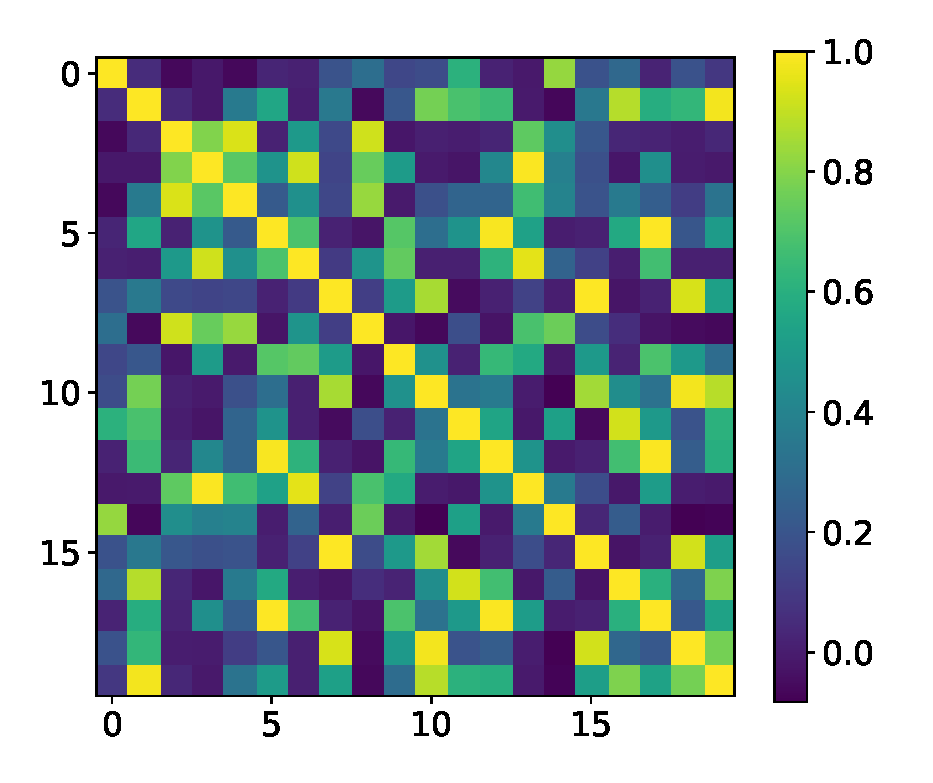
\includegraphics[width=0.9\linewidth]{figs/corr}
			\caption{Correlation matrix}
		\end{figure}
		\end{minipage}
	\begin{block}{Results}
		\begin{itemize}
			\item \# parameters in the initial network: $100 \times 40 + 40 \times 2 = 4080$ (100\%);
			\item accuracy of the initial network: train/test=83.7/78.5;
			\item \# parameters in the reduced network: $92 + 47 = 139$ (4\%);
			\item accuracy of the reduced network: train/test=81.6/78.4
		\end{itemize}
	\end{block}
\end{frame}
%--------------------------------------------------------------------------------
\begin{frame}{Results}
	\begin{block}{Initial network}
		\vspace{-0.2cm}
		\begin{figure}[h]
			\centering
			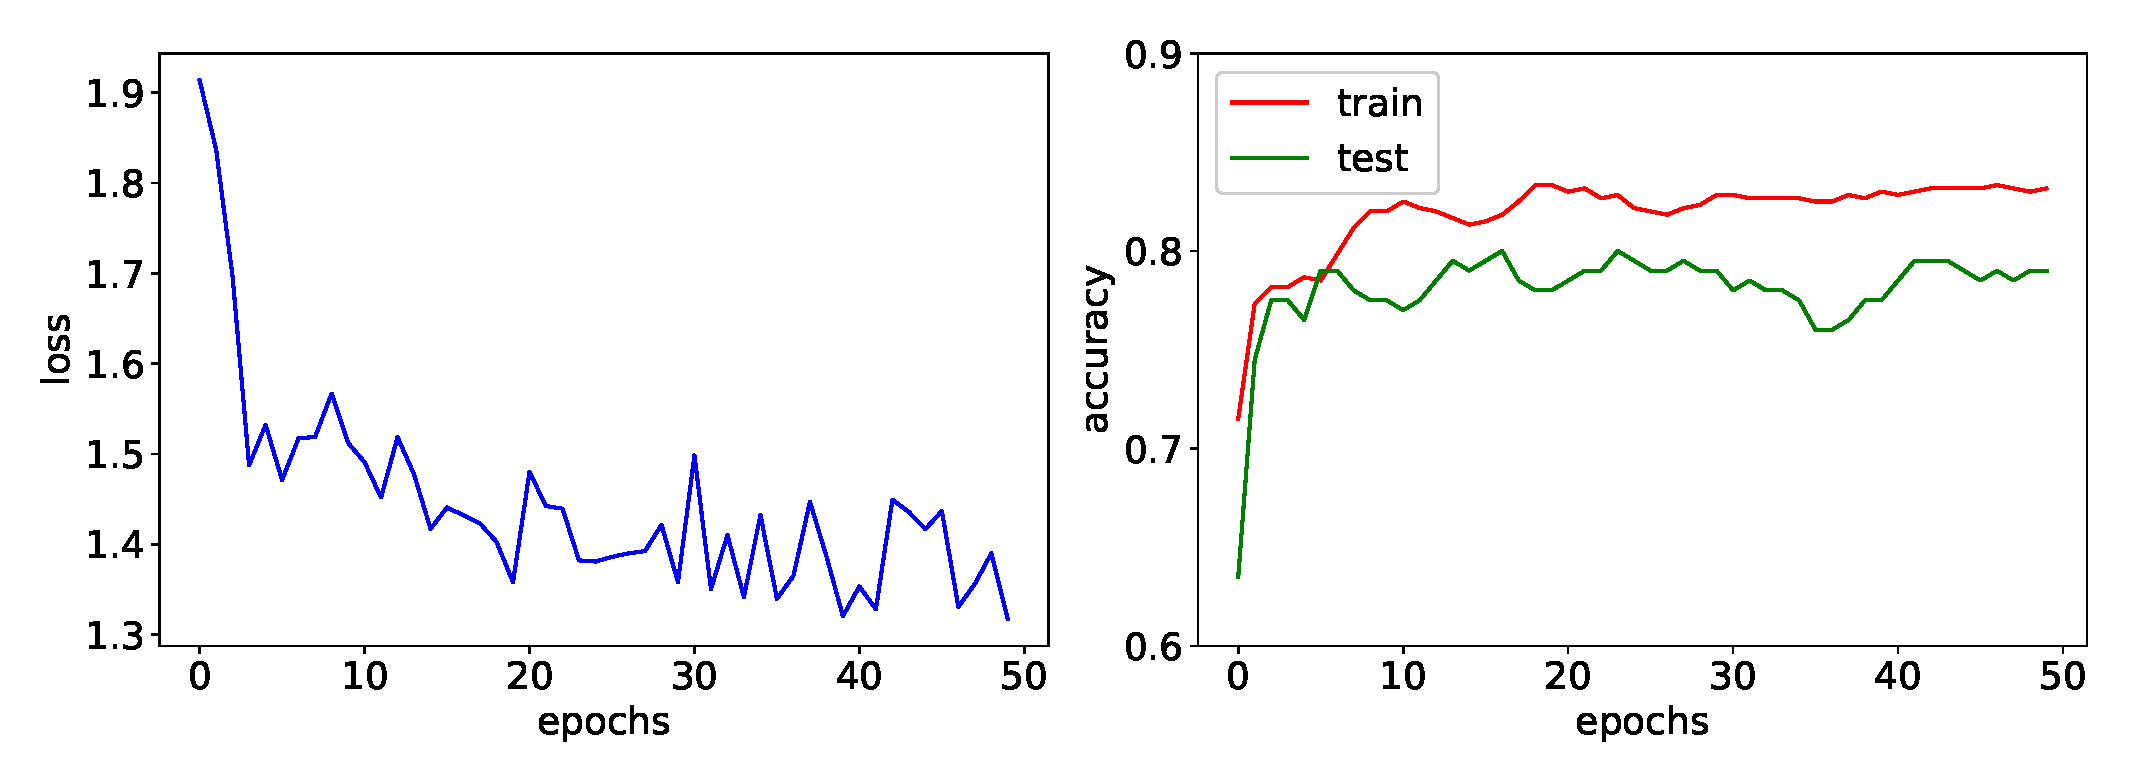
\includegraphics[width=0.9\linewidth]{figs/orig_net.eps}
		\end{figure}
	\end{block}
	\vspace{-0.7cm}
	\begin{block}{Reduced network}
		\vspace{-0.2cm}
		\begin{figure}
			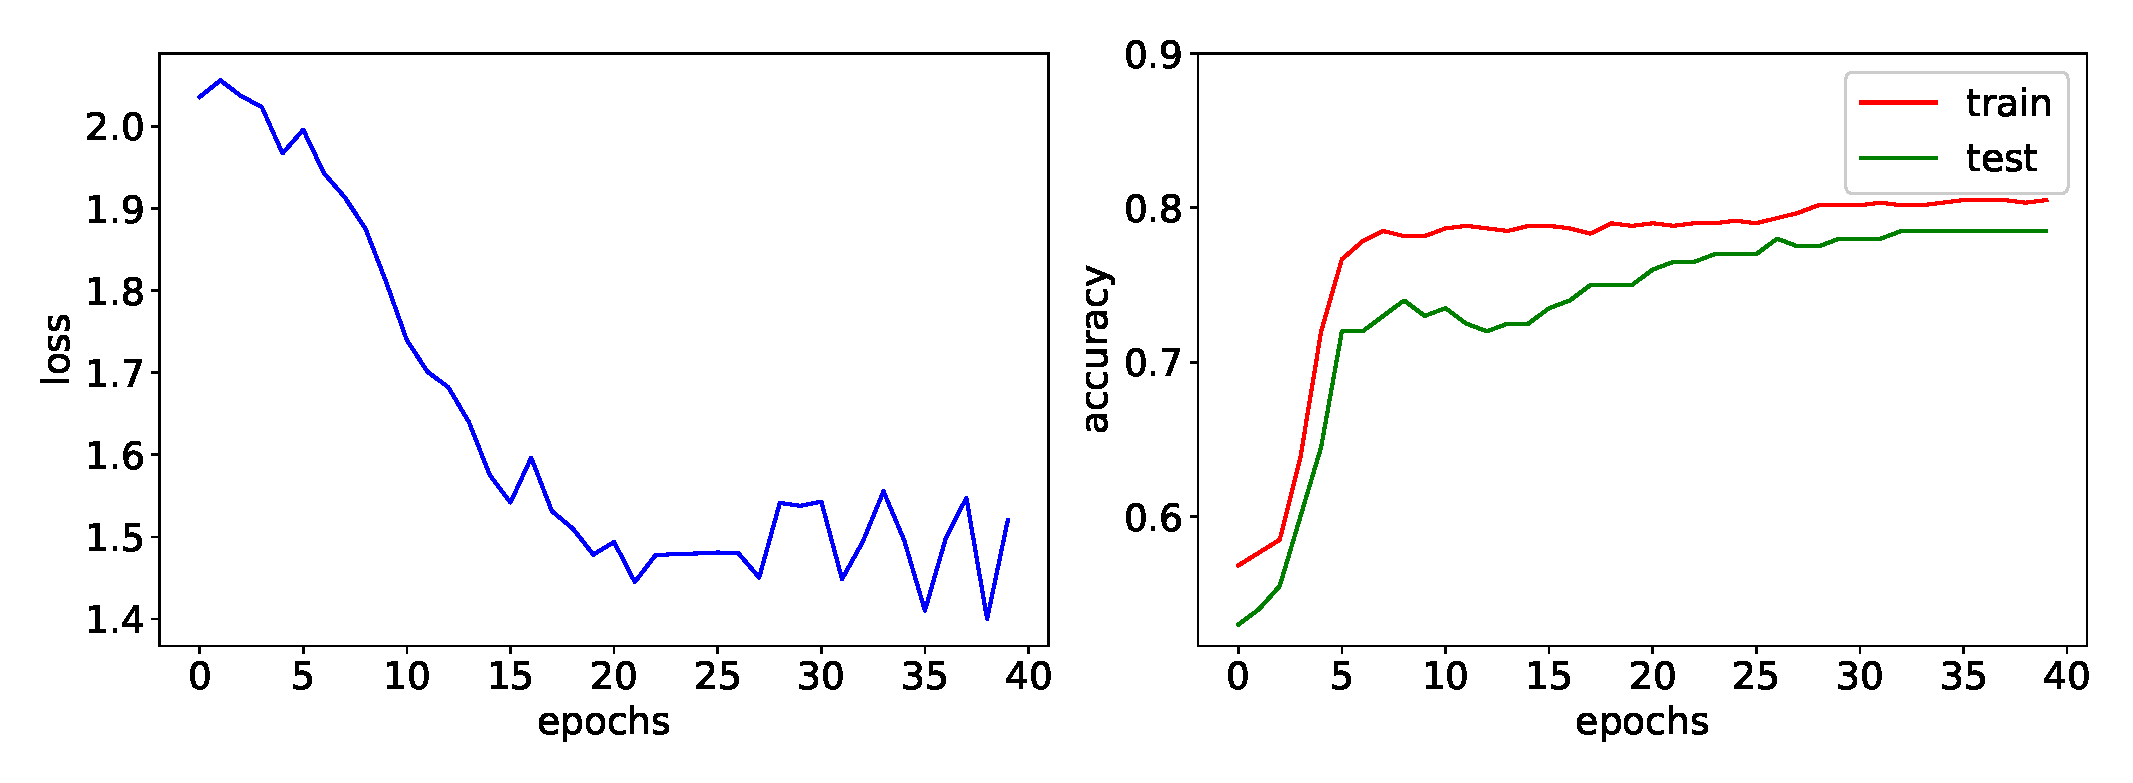
\includegraphics[width=0.9\linewidth]{figs/reduced_net.eps}
		\end{figure}
	\end{block}
\end{frame}
%--------------------------------------------------------------------------------

\end{document} 
